
\documentclass[12pt]{article}
%\usepackage{amsmath}
\usepackage{graphicx}
\usepackage{enumerate}
\usepackage{natbib} %comment out if you do not have the package
\usepackage{url} % not crucial - just used below for the URL 
\usepackage{amsmath, amssymb, amsfonts,calc}
\usepackage{booktabs}
\usepackage{rotating}
\usepackage[section] {placeins}
\usepackage{morefloats}
\usepackage{subcaption}
\usepackage{natbib}
\usepackage{algorithm}
\usepackage{geometry}
\usepackage{algpseudocode}
\usepackage{bm}
\usepackage{caption}
\usepackage{xcolor}
\usepackage[title]{appendix}
\usepackage{float}   % in the preamble
\usepackage{etoc}

%\pdfminorversion=4
% NOTE: To produce blinded version, replace "0" with "1" below.
\newcommand{\blind}{0}

% DON'T change margins - should be 1 inch all around.
\addtolength{\oddsidemargin}{-.5in}%
\addtolength{\evensidemargin}{-1in}%
\addtolength{\textwidth}{1in}%
\addtolength{\textheight}{1.7in}%
\addtolength{\topmargin}{-1in}%

\algrenewcommand\algorithmicindent{0.8em}
% Compact style for tight single-page layout
\algrenewcommand\alglinenumber[1]{\scriptsize #1}
\algrenewcommand\algorithmiccomment[1]{\hfill\textit{// #1}}
\AtBeginEnvironment{algorithmic}{\footnotesize}
\setlength{\textfloatsep}{4pt plus 1pt minus 1pt}
\setlength{\floatsep}{4pt plus 1pt minus 1pt}
\setlength{\intextsep}{4pt plus 1pt minus 1pt}
\setlength{\abovedisplayskip}{4pt}
\setlength{\belowdisplayskip}{4pt}
\renewcommand{\thealgorithm}{A.\arabic{algorithm}} % Appendix numbering


\begin{document}

%\bibliographystyle{natbib}

\def\spacingset#1{\renewcommand{\baselinestretch}%
{#1}\small\normalsize} \spacingset{1}


%%%%%%%%%%%%%%%%%%%%%%%%%%%%%%%%%%%%%%%%%%%%%%%%%%%%%%%%%%%%%%%%%%%%%%%%%%%%%%

\if0\blind
{
  \title{\bf MTL-MICE: Multi-Task Learning in Multiple Imputation by Chained Equation}
  \author{Yuyu Chen\hspace{.2cm}\\
    Yang Feng \\
    Department of Biostatistics, \\
    School of Global Public Health, \\
    New York University}
  \maketitle
} \fi


\if1\blind
{
  \bigskip
  \bigskip
  \bigskip
  \begin{center}
    {\LARGE\bf Title}
\end{center}
  \medskip
} \fi

\bigskip
\begin{abstract}

In the presence of missing data in a set of related datasets, such as multi-region administrative records or repeated survey waves, multiple imputation is affected by the fact that task-specific models do not share information across datasets, while naive pooling can be biased when conditional relationships differ across tasks. We propose MTL-MICE and MTL-MICE+, which are multi-task extensions of multiple imputation by chained equations (MICE). These methods incorporate selective transfer learning into each conditional model within the chained-equation iterations, enhancing the imputation process. For each target task and each variable with missingness, we apply Trans-GLM to identify a set of transferable source tasks by evaluating held-out prediction loss on the target, then fit a high-dimensional generalized linear model using the $\mathcal{A}$-Trans-GLM estimator. MTL-MICE imputes using the pooled transferring-step coefficients, whereas MTL-MICE+ adds a sparse target-specific correction to address mismatch. For continuous outcomes, we calibrate predictive uncertainty by combining bootstrap coefficient draws with an out-of-bag variance estimator using the 0.632 bootstrap rule. Simulations that vary the number of tasks, cross-task transferability, mixed outcome types, clustered task structure, and outlier tasks show that source detection is important for avoiding negative transfer and that the correction step improves robustness as between-task heterogeneity increases. When applied to county-level U.S. election and socio-demographic data organized as state-level tasks, MTL-MICE+ demonstrates stable imputation performance across various missingness rates. It also generates state-to-state transferability networks that summarize empirical similarities between tasks, highlighting its practical utility. Overall, selective transfer within the MICE framework significantly enhances imputation accuracy and maintains robustness in heterogeneous multi-dataset settings, showing its potential for broad application in complex data environments.
\end{abstract}

\noindent%
{\it Keywords:} Multiple imputation; transfer learning; high-dimensional regression; variable selection; out-of-bag error; negative transfer
\vfill

\newpage
\spacingset{1.8} % DON'T change the spacing!
\section{Background}
\label{sec:background}

Missing data is one of the most common challenge in observational studies because it can cause bias and inefficiency in the estimation as well as incorrect conclusions regarding the results of the study \citep{little_statistical_2019,carpenter_multiple_2012}.
These problems can be more complex in high-dimensional settings where many covariates are recorded and missingness can occur across several fields of data sources at once. In the analysis of linked administrative data sets, the missing data can occur because of non-recording as well as errors in the linkage process, which can cause missing data as well as selection bias and misclassification bias \citep{harron_challenges_2017,shaw_biases_2022}.In the analysis of multiple cross-sectional surveys such as the National Health and Nutrition Survey (NHANES), the missing data can vary in the different surveys as well as the characteristics of the respondents in the surveys  \citep{schenker_multiple_2011}. In studies where data is aggregated from multiple sources, missing data issues are often complicated by the fact that different sources have different missing data rates; in a recent systematic review of multi-database pharmaco-epidemiologic studies, only 56\% of studies reported missing data and only 31\% of those studies reported how it was handled \citep{hunt_systematic_2021}.  Our motivating application fits this setting: county-level U.S.\ election results and socio-demographic covariates, aggregated to state-level analytic tasks, are collected from a variety of publicly available sources with different measurement conventions and reporting completeness. If certain variables are more likely to be missing in certain states or counties, the missing data with both cross-variable and cross-task missingness patterns that are difficult to accommodate with methods designed for single-dataset missing data analysis.

One of the most common ways to deal with missing data under reasonable assumptions is by using multiple imputation (MI).MI replaces each missing value with multiple draws from an imputation model, yielding $M$ completed datasets, and then accounting for this imputation uncertainty by applying Rubin’s rules \citep{rubin_multiple_1987,little_statistical_2019}. MI is widely used because it integrates well with most data analysis workflows and provides a framework for incorporating auxiliary data in the imputation model  \citep{schafer_missing_2002,murray_multiple_2018}. However, it is also limited by the performance of the imputation model itself. The imputation model may lead to biases if it is misspecified, and uncertainty may be incorrectly estimated even when MAR is assumed and when omitted conditional dependence is ignored  \citep{meng_multiple-imputation_1994,murray_multiple_2018}.

Multiple imputation by chained equations (MICE) has become a widely used MI strategy \citep{buuren_flexible_2018}. MICE uses a fully conditional specification (FCS): each variable with missing values is imputed from a regression model conditional on the remaining variables, and these models are iteratively cycled to produce multiple completed datasets. Each conditional model can be tailored to the variable type and replaced by any predictive model suitable for that variable.

This flexibility comes at the cost of  methodological choices. Conditional models need to be specified and tuned, and it is not guaranteed that the collection of conditional models supports a coherent joint distribution unless compatibility conditions are met.  Moreover, incompatibility of the imputation model and analysis model may contribute to uncongeniality and impact finite-sample properties of MI estimators\citep{meng_multiple-imputation_1994,bartlett_multiple_2015,murray_multiple_2018}. These problems have been addressed in recent work from different angles. Substantive-model-compatible FCS (SMC-FCS) modifies the chained-equation updates to to ensure compatibility with a user-specified substantive analysis model, which may improve performance when interactions or non-linear terms are needed \citep{bartlett_multiple_2015}. For multilevel and clustered data, extensions of MICE allow systematic missing variables in some clusters and sporadically missing in others \citep{resche-rigon_multiple_2018,enders_multilevel_2016}.
On the modeling side, flexible learners have been incorporated in MICE to reduce misspecification risk. SuperMICE uses an ensemble Super Learner in each chained-equation step
\citep{laqueur_supermice_2022}, and tree-based conditional models such as MICE-CART and MICE-Random Forest are often used to account for non-linearities\citep{doove_recursive_2014,shah_comparison_2014}.
These developments show that MICE is a robust framework, but practical performance depends on how conditional models are constructed, regularized, and calibrated.

\subsection{Missing data in high-dimensional settings}
\label{subsec:background_highdim}

When the number of covariates is large compared to the observed outcomes for a variable being imputed, standard conditional models within MICE may become unstable or infeasible. This instability is due to challenges such as multicollinearity, overfitting, and high computational costs \citep{fan_selective_2010,tibshirani_elements_2009}.A natural solution is to use regularization in the chained-equation regressions, which involves adding a penalty to the regression to prevent overfitting. \citet{deng_multiple_2016} proposed MICE-DURR and
MICE-IURR, which incorporate lasso, elastic net, and adaptive lasso penalties into MICE for general missing-data patterns under high-dimensional covariates.  In a recent study, \citet{brini_missing_2024} compared regularized MI methods in high-dimensional setting and found that indirect use of regularized regression (MICE-IURR) can reduce bias in some settings. \citet{costantini_solving_2023} suggested replacing each conditional regression with principal component regression to stabilize MICE when the pool of predictors is large without variable selection. \citet{varol_review_2025} conducted a systematic review of simulation studies on high-dimensional imputation methods and emphasized the importance of balance in bias, efficiency, and computational costs in choosing a suitable approach for missing data problems in the presence of many covariates.

The other methods directly impose a structure on the data matrix. In matrix completion methods use low-rank assumptions, soft-impute is a popular one, where it is based on an iterative nuclear norm regularization process 
\citep{hastie_matrix_2015,mazumder_spectral_2010}. \citet{lee_high-dimensional_2024} proposed imputation through undirected graphical models, where conditional independence is utilized for the stabilization of the imputation in high-dimensional settings. Deep learning methods, including denoising autoencoders, generative adversarial networks, variational autoencoders, and diffusion models, have also been studied for tabular imputation
\citep{yoon_gain_2018,gondara_mida_2018,tashiro_csdi_2021,du_saits_2023}. In a recent comparative study, \citet{sun_deep_2023} compared different imputation methods and found that for tabular data with moderate-sized samples, MICE and missForest are competitive with or even surpass the performance of deep learning methods, especially for MAR and MNAR mechanisms. This provides motivation to extend the MICE framework rather than replace it.

\subsection{Multi-task and transfer learning}
\label{subsec:background_mtl}

Many datasets are naturally viewed as collections of tasks, where variables are aligned across tasks, such as in multi-center clinical trials, longitudinal studies, multi-region administrative records, and in our case, state-level tasks constructed from county-level measurements. n such cases, we find that two straightforward baselines are often applicable: imputation can be performed separately on each task using separate conditionals, or imputation can be performed by pooling all tasks together and imputing them as a whole, effectively treating them as a single dataset. Task-wise imputation does not share information across tasks, while naive pooling can be biased when tasks differ in their conditional relationships, a setting in which negative transfer is possible \citep{rosenstein_transfer_2005,pan_survey_2010}.

Multi-task learning demonstrates the benefits of learning multiple related tasks jointly, which can reduce the variance of the estimators through the sharing of structure without forcing full pooling \citep{caruana_multitask_1997,ruder_overview_2017}.
\citet{baxter_model_2000} have shown that the joint learning of related tasks can reduce the sample complexity under certain assumptions about the relatedness of the tasks. In regularized regression, the relatedness of the tasks has been captured through the design of penalties that encourage sharing sparsity, low-rank structure, and clustering \citep{yuan_model_2006,pong_trace_2010,zhang_survey_2021}. Transfer learning focuses on the target task and selectively transfers information from a set of source tasks  \citep{pan_survey_2010,zhuang_comprehensive_2021}.
For high-dimensional generalized linear models, \citet{tian_transfer_2022} introduced a transfer-learning framework with a two-step estimator that fits a pooled $\ell_1$-penalized model across selected sources and then estimates a sparse target-specific correction, along with a source-detection procedure that selects informative sources by comparing held-out prediction loss on the target. This combination offers a practical way to borrow information while controlling mismatch.

\subsection{Multi-task and transfer learning for missing-data imputation}
\label{subsec:background_mtl_impute}

Using multi-task and transfer-learning ideas for imputation is natural, but general-purpose methods that integrate these ideas into MI workflows remain limited. In fact, the existing literature has mostly focused on specific types of data. For example, \citet{mcdermott_comprehensive_2020} studied multi-task approaches for electronic health records with temporal structure. \citet{zhou_imputing_2020} used transfer learning to impute missing gene expression values across related tissues. In the domain of spatiotemporal monitoring data, the application of the concept of multi-task learning was explored by \citet{zhu_lane_2025}. In federated and multi-site health data, \citet{li_fedimpute_2025} proposed the method of FedIMPUTE for imputing missing values across hospitals while maintaining the privacy of the data. Deep learning architectures have been used for joint imputation and prediction tasks \citep{lai_autoencoder-based_2021}, but these are typically applied within a single dataset rather than across multiple aligned tasks.

Three gaps motivate our work. Most multi-task imputation methods are tailored to particular data types and do not provide a general framework compatible with MICE. Transferable-source detection, which is important for avoiding negative transfer, has rarely been integrated into imputation workflows.Finally, it remains unclear how selective transfer within imputation affects coefficient recovery and other downstream targets that depend on the conditional models fitted within MICE.

Motivated by \citet{tian_transfer_2022} , we address these gaps by proposing MTL-MICE and MTL-MICE+, multi-task extensions of regularized MICE that integrate selective transfer into each conditional model. For each target task and each variable being imputed, we use Trans-GLM to identify a transferring set of source tasks, then fit $\mathcal{A}$-Trans-GLM to borrow information from the selected sources. MTL-MICE uses the transferring-step coefficients for prediction, while MTL-MICE+ uses the full two-step estimator, including the sparse target correction.
To better calibrate predictive uncertainty for continuous outcomes under shrinkage, we estimate the Gaussian noise variance using an out-of-bag error estimator combined with the 0.632 bootstrap rule proposed by \citealt{efron_improvements_1997}, rather than using training residual variance.

The paper develops the algorithmic framework, evaluates it in simulations that vary the number
of tasks, transferability levels, mixed variable types, clustered task structure, and outlier tasks, and illustrates it on county-level U.S.\ election and socio-demographic data. We also use the Trans-GLM selection output to construct interpretable state-to-state transferability networks, which provide a diagnostic view of empirical similarity between tasks for different variables. The remainder of the paper is organized as follows. Section~\ref{sec:method} presents the proposed methods and conditional models.
Section~\ref{sec:simulation} reports simulation results. Section~\ref{sec:realdata} presents the election case study and transferability networks. Section~\ref{sec:discussion} concludes with limitations and future directions.

\section{Methodology}
\label{sec:method}

\subsection{Notation and data structure}
We consider $K$ related datasets (tasks). Task $k\in\{1,\dots,K\}$ contains a data matrix
$\bm{X}^{(k)}\in\mathbb{R}^{n_k\times p}$ with $n_k$ samples and a common set of $p$ variables.
We write $X^{(k)}_{ij}$ for the $(i,j)$ entry, $\bm{X}^{(k)}_j\in\mathbb{R}^{n_k}$ for the $j$th column,
and $\bm{X}^{(k)}_{-j}\in\mathbb{R}^{n_k\times(p-1)}$ for the matrix with column $j$ removed.

Missingness in task $k$ is encoded by $\bm{R}^{(k)}\in\{0,1\}^{n_k\times p}$, where $R^{(k)}_{ij}=1$
if $X^{(k)}_{ij}$ is observed and $R^{(k)}_{ij}=0$ otherwise. For variable $j$ in task $k$, define
\[
\mathcal{O}^{(k)}_j=\{i:R^{(k)}_{ij}=1\},\qquad
\mathcal{M}^{(k)}_j=\{i:R^{(k)}_{ij}=0\},
\]
and let $|\mathcal{O}^{(k)}_j|$ and $|\mathcal{M}^{(k)}_j|$ be the numbers of observed and missing entries.
For the conditional model used to impute $X^{(k)}_j$, we denote the observed response vector and predictors by
\[
\bm{y}^{(k)}_j=\bm{X}^{(k)}_j[\mathcal{O}^{(k)}_j],\qquad
\bm{Z}^{(k)}_j=\bm{X}^{(k)}_{-j}[\mathcal{O}^{(k)}_j].
\]

Let $M$ be the number of multiply imputed datasets and $T$ the number of chained-equation iterations within each imputation.
To avoid confusion with the number of incomplete variables used later in simulations, we index imputations by $q\in\{1,\dots,M\}$.
We write $\bm{X}^{(k,q,t)}$ for the current filled-in version of task $k$ at iteration $t\in\{0,\dots,T\}$ within imputation $q$,
where $t=0$ denotes initialization. When imputing entries in $\mathcal{M}^{(k)}_j$ at iteration $t$, the predictors are taken from the
current iterate $\bm{X}^{(k,q,t-1)}_{-j}[\mathcal{M}^{(k)}_j]$, so each update uses the latest values of the other variables.

\subsection{Lasso-based multiple imputation by chained equations (DURR-MICE)}
\label{subsec:durr_mice}
Multiple imputation replaces each missing value by multiple draws from a predictive distribution, producing $M$ completed datasets,
and combines downstream estimates using Rubin's rules \citep{rubin_multiple_1987}. MICE implements this idea for general missingness
patterns by specifying conditional models $\{f_j(X_j\mid \bm{X}_{-j};\theta_j)\}_{j=1}^p$ and iterating through $j=1,\dots,p$,
updating the missing entries of each variable using the current filled-in values of the remaining variables \citep{buuren_flexible_2018}. Algorithm ~\ref{alg:mice} shows the detailed MICE procedure.

In high-dimensional settings, classical regression imputation can be unstable when the number of candidate predictors is large relative to
the number of complete cases for the outcome being imputed. We use the direct use of regularized regression strategy as a benchmark,
embedding lasso-regularized GLMs within MICE and using bootstrap resampling to generate stochastic coefficient draws \citep{deng_multiple_2016}.
Fix task $k$ and variable $j$ with $\mathcal{M}^{(k)}_j\neq\emptyset$, and define $(\bm{Z}^{(k)}_j,\bm{y}^{(k)}_j)$ on the complete cases
$\mathcal{O}^{(k)}_j$ as above. We draw bootstrap indices $\mathcal{I}^{(k)}_j$ by sampling $|\mathcal{O}^{(k)}_j|$ elements with replacement
from $\mathcal{O}^{(k)}_j$, and fit a lasso-penalized GLM (intercept unpenalized) on the bootstrap sample. Writing $\psi(\cdot)$ for the GLM
cumulant function and augmenting predictors with an intercept column $\tilde{\bm{Z}}=[\bm{1},\bm{Z}]$, the fitted coefficient vector is
\[
\hat{\bm{\beta}}^{(k)}_j
=\arg\min_{\bm{\beta}}
\left\{
\frac{1}{|\mathcal{I}^{(k)}_j|}
\sum_{i\in\mathcal{I}^{(k)}_j}\big[-y_i\,\tilde{\bm{z}}_i^\top\bm{\beta}+\psi(\tilde{\bm{z}}_i^\top\bm{\beta})\big]
+\lambda\|\bm{\beta}_{-0}\|_1
\right\},
\]
where $\bm{\beta}_{-0}$ excludes the intercept coefficient. This bootstrap fit provides a stochastic draw of regression parameters within the
MICE iterations.

For imputing rows $i\in\mathcal{M}^{(k)}_j$, let $\tilde{\bm{Z}}^{(k,q,t-1)}_{j,\mathrm{mis}}=[\bm{1},\bm{X}^{(k,q,t-1)}_{-j}[\mathcal{M}^{(k)}_j]]$
and define the linear predictor $\hat{\bm{\eta}}=\tilde{\bm{Z}}^{(k,q,t-1)}_{j,\mathrm{mis}}\hat{\bm{\beta}}^{(k)}_j$.
For a binary $X^{(k)}_j$, we set $p_i=\mathrm{logit}^{-1}(\hat{\eta}_i)$ and draw $X^{(k,q,t)}_{ij}\sim\mathrm{Bernoulli}(p_i)$ independently.
For a continuous $X^{(k)}_j$, we draw $X^{(k,q,t)}_{ij}=\hat{\eta}_i+\varepsilon_i$ with $\varepsilon_i\sim\mathcal{N}(0,\hat{\sigma}^2)$.
In this paper, $\hat{\sigma}^2$ is estimated by an out-of-bag mean squared error combined with the 0.632 bootstrap rule, as described in
Section~\ref{subsec:mtlmice_implementation}, and the same variance estimator is used across methods to keep predictive-noise calibration comparable.

\subsection{Transfer learning under high-dimensional generalized linear models}
\label{subsec:glmtrans}
Our multi-task imputation uses the transfer-learning framework of \citet{tian_transfer_2022}, implemented in the \texttt{glmtrans} R package.
The goal is to estimate a target-task GLM coefficient vector by borrowing information from source tasks when this improves target prediction,
while reducing the risk of negative transfer when sources are mismatched. The framework consists of a two-step estimator that conditions on a
chosen set of source tasks, and a source-detection procedure that selects such tasks using target held-out loss \citep{tian_transfer_2022}.

For each task $k$, consider a GLM with density
\[
\mathbb{P}(y^{(k)}\mid \bm{x}^{(k)}) \propto \rho(y^{(k)})\exp\left\{y^{(k)}(\bm{x}^{(k)})^\top \bm{\beta}^{(k)}-\psi\!\left((\bm{x}^{(k)})^\top \bm{\beta}^{(k)}\right)\right\},
\]
where $\psi(\cdot)$ is the cumulant function and $\psi'(\cdot)$ is the mean function. We include an intercept by augmenting predictors with
a leading 1, written as $\tilde{\bm{x}}=(1,\bm{x}^\top)^\top$ and $\tilde{\bm{Z}}=[\bm{1},\bm{Z}]$. In our imputation setting we use
Gaussian and logistic families.

\paragraph{Task relatedness for a single conditional model.}
Fix a target task $k$ and variable $j$. Let $\bm{\beta}^{(k)}_j$ denote the coefficient vector for the conditional model of $X^{(k)}_j$
given $\bm{X}^{(k)}_{-j}$ (including the intercept). For a candidate source task $\ell\neq k$, let $\bm{w}^{(\ell)}_j$ denote the
corresponding coefficient vector and define the contrast
\(\bm{\delta}^{(\ell\to k)}_j=\bm{\beta}^{(k)}_j-\bm{w}^{(\ell)}_j.\)
A common way to formalize transferability is to say that source $\ell$ is transferable to target $k$ at level $h$ for variable $j$ if
$\|\bm{\delta}^{(\ell\to k)}_j\|_1\le h$. The set of transferable sources is then
\[
\mathcal{A}^{(k)}_{j,h}=\left\{\ell\in\{1,\dots,K\}\setminus\{k\}:\ \|\bm{\delta}^{(\ell\to k)}_j\|_1\le h\right\}.
\]
In applications, $\mathcal{A}^{(k)}_{j,h}$ is unknown and is estimated by Trans-GLM; we denote the estimated set by $\widehat{\mathcal{A}}^{(k)}_j$.
The penalties $\lambda_w$ and $\lambda_\delta$ are used for the pooled transferring step and the target correction step, respectively, and Trans-GLM
uses a threshold constant $C_0>0$ together with a small $\epsilon_0>0$.

\subsubsection{$\mathcal{A}$-Trans-GLM: transferring and target correction}
\label{subsubsec:atransglm}
Fix a target task indexed by $0$ with data $(\bm{X}^{(0)},\bm{y}^{(0)})$ and a set of source tasks $\mathcal{A}\subseteq\{1,\dots,K\}$
with data $\{(\bm{X}^{(k)},\bm{y}^{(k)})\}_{k\in\mathcal{A}}$. $\mathcal{A}$-Trans-GLM estimates the target coefficients in two steps.

The transferring step fits a pooled lasso GLM on the union of target and source data:
\[
\hat{\bm{w}}^{\mathcal{A}}
=\arg\min_{\bm{w}}
\left\{
\frac{1}{n_0+n_{\mathcal{A}}}\sum_{k\in\{0\}\cup\mathcal{A}}
\Big[-(\bm{y}^{(k)})^\top \bm{X}^{(k)}\bm{w}+\sum_{i=1}^{n_k}\psi(\bm{w}^\top \bm{x}^{(k)}_i)\Big]
+\lambda_w\|\bm{w}\|_1
\right\}.
\]
This step reduces variance by increasing the effective sample size, but it can be biased when some sources are far from the target.

The correction step estimates a sparse target-specific adjustment using target data only:
\[
\hat{\bm{\delta}}^{\mathcal{A}}
=\arg\min_{\bm{\delta}}
\left\{
-\frac{1}{n_0}(\bm{y}^{(0)})^\top \bm{X}^{(0)}(\hat{\bm{w}}^{\mathcal{A}}+\bm{\delta})
+\frac{1}{n_0}\sum_{i=1}^{n_0}\psi\!\left((\hat{\bm{w}}^{\mathcal{A}}+\bm{\delta})^\top \bm{x}^{(0)}_i\right)
+\lambda_\delta\|\bm{\delta}\|_1
\right\},
\qquad
\hat{\bm{\beta}}=\hat{\bm{w}}^{\mathcal{A}}+\hat{\bm{\delta}}^{\mathcal{A}}.
\]
\citet{tian_transfer_2022} recommend penalties that scale with $\sqrt{\log(p)/n}$, with different effective sample sizes in the two steps.
One representative form is
\[
\lambda_w=C_w\left(\sqrt{\frac{\log p}{n_{\mathcal{A}}+n_0}}+h\right),\qquad
\lambda_\delta=C_\delta\sqrt{\frac{\log p}{n_0}},
\]
where $h$ represents a source-target discrepancy level. Algorithm~\ref{alg:atransglm} shows the detailed $\mathcal{A}$-Trans-GLM procedure.

In our implementation, \texttt{glmtrans} fits a lasso path using \texttt{glmnet} with mixing parameter $\alpha=1$ and chooses penalties by
cross-validation. The package defaults use \texttt{lambda.1se} for the transferring step and for Trans-GLM detection, and \texttt{lambda.min}
for the correction step. In all MTL-MICE experiments in this paper, we also use \texttt{lambda.1se} for the correction step. This choice
reduces variance in the correction fit, which is repeatedly re-estimated inside the chained-equation iterations and on bootstrap resamples,
and it avoids unstable corrections that can propagate through subsequent MICE updates.

\subsubsection{Trans-GLM: transferable source detection}
\label{subsubsec:transglm}
When $\mathcal{A}$ is unknown, Trans-GLM estimates a transferring set by comparing target held-out loss with and without each candidate source.
For the target task, split the observed index set into three folds and, for each fold $r$, fit a target-only lasso GLM on the other two folds
to obtain $\hat{\bm{\beta}}^{(0)[r]}$. For each source task $k$, fit only the transferring step using the same two target folds pooled with
source $k$ to obtain $\hat{\bm{\beta}}^{(k)[r]}$. Evaluate negative log-likelihood loss on the held-out fold to form $\widehat{L}_0^{[r]}(\hat{\bm{\beta}}^{(k)[r]})$.
Aggregating across folds yields
\[
\widehat{L}^{(k)}_0=\frac{1}{3}\sum_{r=1}^3 \widehat{L}^{[r]}_0(\hat{\bm{\beta}}^{(k)[r]}),\qquad
\widehat{L}^{(0)}_0=\frac{1}{3}\sum_{r=1}^3 \widehat{L}^{[r]}_0(\hat{\bm{\beta}}^{(0)[r]}).
\]
Let
\[
\hat{\sigma}=\sqrt{\frac{1}{2}\sum_{r=1}^3\Big(\widehat{L}^{[r]}_0(\hat{\bm{\beta}}^{(0)[r]})-\widehat{L}^{(0)}_0\Big)^2 }.
\]
Trans-GLM selects sources whose excess loss is below a threshold:
\[
\widehat{\mathcal{A}}=\Big\{k\neq 0:\ \widehat{L}^{(k)}_0-\widehat{L}^{(0)}_0 \le C_0\big(\hat{\sigma}\vee \epsilon_0\big)\Big\},
\]
with $\epsilon_0$ set to $0.01$ in our experiments. The selected set $\widehat{\mathcal{A}}$ is then used in $\widehat{\mathcal{A}}$-Trans-GLM
to produce a transferred estimate. \citet{tian_transfer_2022} also discuss penalty scaling for detection fits; in \texttt{glmtrans} these penalties
are chosen by cross-validation and, in our implementation, use \texttt{lambda.1se} with three-fold validation to match the detection procedure. 

A useful comparator is the pooled variant that sets $\mathcal{A}=\{1,\dots,K\}$ and runs $\mathcal{A}$-Trans-GLM without source detection.
This can perform well when most sources are close to the target, but it can be harmed by negative transfer when only a subset of sources are compatible.

\subsection{MTL-MICE and MTL-MICE+}
\label{subsec:mtlmice_implementation}

Our proposed MTL-MICE and MTL-MICE+ extend multiple imputation by chained equations (MICE) to collections of related datasets by incorporating selective transfer learning into each conditional model. The methods keep the chained-equation updates used for general missingness patterns, introduce between-imputation variation through bootstrap coefficient draws as in regularized MI, and borrow information across tasks through \texttt{glmtrans} when source tasks are estimated to improve prediction for a target task. We index the $M$ multiply imputed datasets by $q\in\{1,\dots,M\}$ and the MICE iterations by $t\in\{1,\dots,T\}$. Within each replicate $q$, the algorithm cycles through tasks $k=1,\dots,K$ and variables $j$ with $\mathcal{M}^{(k)}_j\neq\emptyset$, updating the missing entries in column $j$ of task $k$ from a conditional GLM given the current values of the remaining variables.

Fix an update at replicate $q$, iteration $t$, task $k$, and variable $j$. The target complete-case training data for imputing $X^{(k)}_j$ is formed from the current filled-in matrix $\bm{X}^{(k,q,t-1)}$:
\[
\bm{y}^{(k)}_{j}=\bm{X}^{(k,q,t-1)}_{j}[\mathcal{O}^{(k)}_j],\qquad
\bm{Z}^{(k)}_{j}=\bm{X}^{(k,q,t-1)}_{-j}[\mathcal{O}^{(k)}_j].
\]
For each candidate source task $\ell\neq k$, we define the corresponding complete-case data using $\bm{X}^{(\ell,q,t-1)}$:
\[
\bm{y}^{(\ell)}_{j}=\bm{X}^{(\ell,q,t-1)}_{j}[\mathcal{O}^{(\ell)}_j],\qquad
\bm{Z}^{(\ell)}_{j}=\bm{X}^{(\ell,q,t-1)}_{-j}[\mathcal{O}^{(\ell)}_j].
\]
Because updates proceed sequentially within MICE, the predictor matrices $\bm{Z}^{(k)}_j$ and $\bm{Z}^{(\ell)}_j$ may contain values imputed earlier in the same iteration, as in standard chained equations (Algorithm~\ref{alg:mtlmice_outer}).

To represent parameter uncertainty within each conditional model, we use bootstrap resampling over the observed indices of the outcome being imputed. For each task $\ell$ used in the update, we sample bootstrap indices
\(\mathcal{I}^{(\ell)}_{j}\ \text{as a size-}|\mathcal{O}^{(\ell)}_j|\ \text{sample with replacement from } \mathcal{O}^{(\ell)}_j,\)
and fit the conditional model using $(\bm{Z}^{(\ell)}_{j}[\mathcal{I}^{(\ell)}_{j}],\bm{y}^{(\ell)}_{j}[\mathcal{I}^{(\ell)}_{j}])$ (Algorithm~\ref{alg:atransglm_boot}). This yields a stochastic coefficient draw at each chained update and each imputation replicate.

Borrowing across tasks is controlled by a transferring set $\widehat{\mathcal{A}}^{(k)}_j\subseteq\{1,\dots,K\}\setminus\{k\}$ (Algorithm~\ref{alg:transglm_detect}). In the default setting, $\widehat{\mathcal{A}}^{(k)}_j$ is estimated by Trans-GLM source detection using a 3-fold split of the target complete cases, retaining sources whose inclusion does not increase the target held-out loss beyond a threshold (Section~\ref{subsubsec:transglm}). For comparison, we also consider the pooled choice $\widehat{\mathcal{A}}^{(k)}_j=\{1,\dots,K\}\setminus\{k\}$, which uses all other tasks as sources without detection, and the no-transfer choice $\widehat{\mathcal{A}}^{(k)}_j=\emptyset$, which reduces the update to a target-only lasso conditional model (denote as Local-MICE in Section \ref{sec:simulation}, which is the analogue of Lasso-based DURR-MICE).

Conditional model estimation depends on whether sources are selected. If $\widehat{\mathcal{A}}^{(k)}_j=\emptyset$, we fit a target-only lasso GLM on the bootstrap target sample to obtain $\hat{\bm{\beta}}^{(k)}_j$. If $\widehat{\mathcal{A}}^{(k)}_j\neq\emptyset$, we fit $\widehat{\mathcal{A}}^{(k)}_j$-Trans-GLM. Writing $\psi(\cdot)$ for the GLM cumulant function, the transferring step estimates pooled coefficients
\[
\hat{\bm{w}}^{\widehat{\mathcal{A}}}
=\arg\min_{\bm{w}}
\left\{
\frac{1}{n_k+n_{\widehat{\mathcal{A}}}}\sum_{\ell\in\{k\}\cup \widehat{\mathcal{A}}^{(k)}_j}
\Big[-(\bm{y}^{(\ell)}_j)^\top \bm{Z}^{(\ell)}_{j}\bm{w}
      + \sum_{i}\psi(\bm{w}^\top \bm{z}^{(\ell)}_{j,i})\Big]
+ \lambda_w\|\bm{w}\|_1
\right\},
\]
and the correction step estimates a sparse target adjustment using target data,
\[
\hat{\bm{\delta}}^{\widehat{\mathcal{A}}}
=\arg\min_{\bm{\delta}}
\left\{
-\frac{1}{n_k}(\bm{y}^{(k)}_j)^\top \bm{Z}^{(k)}_{j}(\hat{\bm{w}}^{\widehat{\mathcal{A}}}+\bm{\delta})
+\frac{1}{n_k}\sum_{i}\psi\!\left((\hat{\bm{w}}^{\widehat{\mathcal{A}}}+\bm{\delta})^\top \bm{z}^{(k)}_{j,i}\right)
+ \lambda_\delta\|\bm{\delta}\|_1
\right\}.
\]
MTL-MICE uses the transferring-step coefficients for prediction, setting $\hat{\bm{\beta}}^{(k)}_j=\hat{\bm{w}}^{\widehat{\mathcal{A}}}$, while MTL-MICE+ uses the corrected coefficients $\hat{\bm{\beta}}^{(k)}_j=\hat{\bm{w}}^{\widehat{\mathcal{A}}}+\hat{\bm{\delta}}^{\widehat{\mathcal{A}}}$. The two methods therefore differ only in whether the correction term is used when generating imputations, with the same transferring set $\widehat{\mathcal{A}}^{(k)}_j$ and the same bootstrap scheme.


% ==========================================
%  (B) Bootstrap A-Trans-GLM fit (glmtrans)
% ==========================================
\begin{algorithm}[H]
\footnotesize
\caption{Bootstrap $\widehat{\mathcal{A}}$-Trans-GLM fit for a single conditional model $(k,j)$}
\label{alg:atransglm_boot}
\textbf{Input:} Target complete-case data $(\bm{Z}^{(k)}_j,\bm{y}^{(k)}_j)$; sources
$\{(\bm{Z}^{(\ell)}_j,\bm{y}^{(\ell)}_j)\}_{\ell\in\widehat{\mathcal{A}}^{(k)}_j}$; bootstrap indices
$\mathcal{I}^{(\ell)}_j$ sampled from $\mathcal{O}^{(\ell)}_j$; penalties $(\lambda_w,\lambda_\delta)$;
correction flag $\in\{\texttt{off},\texttt{on}\}$; cumulant $\psi(\cdot)$.\\
\textbf{Output:} coefficient draw $\hat{\bm{\beta}}^{(k)}_j$ and OOB set $\mathcal{OOB}^{(k)}_j$.
\begin{algorithmic}[1]
\State For each $\ell\in\{k\}\cup\widehat{\mathcal{A}}^{(k)}_j$, form bootstrapped samples
$(\bm{Z}^{(\ell)}_{j,\mathrm{boot}},\bm{y}^{(\ell)}_{j,\mathrm{boot}})
\leftarrow (\bm{Z}^{(\ell)}_j[\mathcal{I}^{(\ell)}_j],\bm{y}^{(\ell)}_j[\mathcal{I}^{(\ell)}_j])$.
\State Define the effective pooled complete-case size for variable $j$:
\[
n_{\widehat{\mathcal{A}},j}\leftarrow \sum_{\ell\in\widehat{\mathcal{A}}^{(k)}_j}|\mathcal{O}^{(\ell)}_j|.
\]
\State \textbf{Step 1 (transferring / pooled lasso GLM):}
\[
\hat{\bm{w}} \leftarrow \arg\min_{\bm{w}}
\Bigg\{
\frac{1}{|\mathcal{O}^{(k)}_j|+n_{\widehat{\mathcal{A}},j}}
\sum_{\ell\in\{k\}\cup\widehat{\mathcal{A}}^{(k)}_j}
\sum_{i\in \mathcal{I}^{(\ell)}_j}
\Big[-y^{(\ell)}_{j,i}\,\bm{z}^{(\ell)\top}_{j,i}\bm{w}
+\psi\!\big(\bm{z}^{(\ell)\top}_{j,i}\bm{w}\big)\Big]
+\lambda_w\|\bm{w}\|_1
\Bigg\}.
\]
\If{correction flag = \texttt{on}}
  \State \textbf{Step 2 (target correction / sparse contrast):}
  \[
  \hat{\bm{\delta}} \leftarrow \arg\min_{\bm{\delta}}
  \Bigg\{
  \frac{1}{|\mathcal{O}^{(k)}_j|}\sum_{i\in \mathcal{I}^{(k)}_j}
  \Big[-y^{(k)}_{j,i}\,\bm{z}^{(k)\top}_{j,i}(\hat{\bm{w}}+\bm{\delta})
      +\psi\!\big(\bm{z}^{(k)\top}_{j,i}(\hat{\bm{w}}+\bm{\delta})\big)\Big]
  +\lambda_\delta\|\bm{\delta}\|_1
  \Bigg\},
  \qquad \hat{\bm{\beta}}^{(k)}_j\leftarrow \hat{\bm{w}}+\hat{\bm{\delta}}.
  \]
\Else
  \State $\hat{\bm{\beta}}^{(k)}_j\leftarrow \hat{\bm{w}}$.
\EndIf
\State Let $\mathcal{I}^{(k)\ast}_j$ be the unique indices in $\mathcal{I}^{(k)}_j$ and set
$\mathcal{OOB}^{(k)}_j \leftarrow \mathcal{O}^{(k)}_j \setminus \mathcal{I}^{(k)\ast}_j$.
\end{algorithmic}
\end{algorithm}

Given $\hat{\bm{\beta}}^{(k)}_j$, we generate predictive draws for the missing entries. Let
\[
\tilde{\bm{Z}}^{(k,q,t-1)}_{j,\mathrm{mis}}
=\big[\bm{1},\ \bm{X}^{(k,q,t-1)}_{-j}[\mathcal{M}^{(k)}_j]\big],
\qquad
\hat{\bm{\eta}}=\tilde{\bm{Z}}^{(k,q,t-1)}_{j,\mathrm{mis}}\hat{\bm{\beta}}^{(k)}_j.
\]
If $X^{(k)}_j$ is binary, we set $p_i=\mathrm{logit}^{-1}(\hat{\eta}_i)$ and draw $X^{(k,q,t)}_{ij}\sim\mathrm{Bernoulli}(p_i)$ independently for $i\in\mathcal{M}^{(k)}_j$. If $X^{(k)}_j$ is continuous, we draw
\[
X^{(k,q,t)}_{ij}=\hat{\eta}_i+\varepsilon_i,\qquad
\varepsilon_i\overset{\text{i.i.d.}}{\sim}\mathcal{N}(0,\hat{\sigma}^2_{kjt}),
\quad i\in\mathcal{M}^{(k)}_j,
\]
and the remaining choice is the variance estimator $\hat{\sigma}^2_{kjt}$. Algorithm ~\ref{alg:one_update} shows the detailed one chained-equation update of the proposed methods.

% ==========================================
%  (C) One chained update: draw + impute
% ==========================================
\begin{algorithm}[t]
\footnotesize
\caption{One chained-equation update for task $k$, variable $j$ at $(q,t)$}
\label{alg:one_update}
\textbf{Input:} current filled-in data $\bm{X}^{(\cdot,q,t-1)}$; $(k,j)$ with $\mathcal{M}^{(k)}_j\neq\emptyset$;
source mode $\in\{\texttt{auto},\texttt{all},\texttt{none}\}$; correction flag $\in\{\texttt{off},\texttt{on}\}$;
penalties $(\lambda_w,\lambda_\delta)$; OOB minimum size $n_{\min}$.\\
\textbf{Output:} updated $\bm{X}^{(k,q,t)}_j[\mathcal{M}^{(k)}_j]$.
\begin{algorithmic}[1]
\State Form target complete-case data:
$\bm{y}^{(k)}_{j}\leftarrow \bm{X}^{(k,q,t-1)}_j[\mathcal{O}^{(k)}_j]$,
$\bm{Z}^{(k)}_{j}\leftarrow \bm{X}^{(k,q,t-1)}_{-j}[\mathcal{O}^{(k)}_j]$;
and sources $(\bm{y}^{(\ell)}_j,\bm{Z}^{(\ell)}_j)$ analogously for $\ell\neq k$.
\If{source mode = \texttt{auto}}
  \State $\widehat{\mathcal{A}}^{(k)}_j \leftarrow \text{Alg.~\ref{alg:transglm_detect}}(\bm{Z}^{(k)}_j,\bm{y}^{(k)}_j,\{(\bm{Z}^{(\ell)}_j,\bm{y}^{(\ell)}_j)\})$.
\ElsIf{source mode = \texttt{all}}
  \State $\widehat{\mathcal{A}}^{(k)}_j \leftarrow \{1,\dots,K\}\setminus\{k\}$.
\Else
  \State $\widehat{\mathcal{A}}^{(k)}_j \leftarrow \emptyset$.
\EndIf
\State Draw bootstrap indices $\mathcal{I}^{(\ell)}_j$ from $\mathcal{O}^{(\ell)}_j$ for each $\ell\in\{k\}\cup\widehat{\mathcal{A}}^{(k)}_j$.
\If{$\widehat{\mathcal{A}}^{(k)}_j=\emptyset$}
  \State Fit target-only lasso GLM on $(\bm{Z}^{(k)}_j[\mathcal{I}^{(k)}_j],\bm{y}^{(k)}_j[\mathcal{I}^{(k)}_j])$ to obtain $\hat{\bm{\beta}}^{(k)}_j$.
  \State Set $\mathcal{OOB}^{(k)}_j$ from the bootstrap indices as in Alg.~\ref{alg:atransglm_boot}.
\Else
  \State $(\hat{\bm{\beta}}^{(k)}_j,\mathcal{OOB}^{(k)}_j)\leftarrow \text{Alg.~\ref{alg:atransglm_boot}}(\widehat{\mathcal{A}}^{(k)}_j,\{\mathcal{I}^{(\ell)}_j\},\lambda_w,\lambda_\delta,\text{correction flag})$.
\EndIf
\State Compute linear predictor on missing rows. Let $\tilde{\bm{Z}}^{(k)}_{j,\mathrm{mis}}\leftarrow [\bm{1},\ \bm{X}^{(k,q,t-1)}_{-j}[\mathcal{M}^{(k)}_j]]$ and
$\hat{\bm{\eta}}\leftarrow \tilde{\bm{Z}}^{(k)}_{j,\mathrm{mis}}\hat{\bm{\beta}}^{(k)}_j$.
\If{$X^{(k)}_j$ is binary}
  \State $p_i\leftarrow \mathrm{logit}^{-1}(\hat{\eta}_i)$; draw $X^{(k,q,t)}_{ij}\sim\mathrm{Bernoulli}(p_i)$ for $i\in\mathcal{M}^{(k)}_j$.
\Else
  \State \textbf{OOB-.632 variance:} define in-bag unique indices $\mathcal{I}^{(k)\ast}_j$ and
  $\mathcal{OOB}^{(k)}_j=\mathcal{O}^{(k)}_j\setminus\mathcal{I}^{(k)\ast}_j$.
  Compute
  \[
\widehat{\mathrm{MSE}}_{\mathrm{in}}=\frac{1}{|\mathcal{I}^{(k)\ast}_j|}\sum_{i\in\mathcal{I}^{(k)\ast}_j}\big(y^{(k)}_{j,i}-\hat{y}^{(k)}_{j,i}\big)^2,\quad
\widehat{\mathrm{MSE}}_{\mathrm{oob}}=\frac{1}{|\mathcal{OOB}^{(k)}_j|}\sum_{i\in\mathcal{OOB}^{(k)}_j}\big(y^{(k)}_{j,i}-\hat{y}^{(k)}_{j,i}\big)^2.
\]
  Set
  \[
  \hat{\sigma}^2 \leftarrow
  \begin{cases}
    0.368\,\widehat{\mathrm{MSE}}_{\mathrm{in}} + 0.632\,\widehat{\mathrm{MSE}}_{\mathrm{oob}}, & |\mathcal{OOB}^{(k)}_j|\ge n_{\min},\\
    \widehat{\mathrm{MSE}}_{\mathrm{in}}, & \text{otherwise}.
  \end{cases}
  \]
  \State Draw $X^{(k,q,t)}_{ij}=\hat{\eta}_i+\varepsilon_i$, $\varepsilon_i\sim\mathcal{N}(0,\hat{\sigma}^2)$ for $i\in\mathcal{M}^{(k)}_j$.
\EndIf
\end{algorithmic}
\end{algorithm}

\paragraph{Proposed resampling uncertainty: out-of-bag (OOB) variance with a .632 correction.} In regression imputation, $\hat{\sigma}^2$ is often taken from an OLS residual variance, from a Bayesian linear regression model, or from the training mean squared error of the fitted model. These training-based estimates evaluate error on the same cases used for fitting, so they tend to be optimistic for prediction, especially after model selection and shrinkage \citep{breiman_out--bag_1996}. In high-dimensional MICE updates, this optimism typically yields predictive noise that is too small, which produces under-dispersed imputations and can affect later chained updates because imputed values enter as predictors.

To reduce this effect, we estimate predictive variance using out-of-bag (OOB) error from the same bootstrap resample that generates the coefficient draw. Let $\mathcal{I}^{(k)}_j$ be the bootstrap index multiset drawn from $\mathcal{O}^{(k)}_j$, let $\mathcal{I}^{(k)\ast}_j$ be the set of unique in-bag indices, and define the OOB set
\(\mathcal{OOB}^{(k)}_j=\mathcal{O}^{(k)}_j\setminus \mathcal{I}^{(k)\ast}_j.\)
Using fitted values from the bootstrap-trained conditional model, we compute
\[
\widehat{\mathrm{MSE}}_{\mathrm{in}}
=\frac{1}{|\mathcal{I}^{(k)\ast}_j|}\sum_{i\in \mathcal{I}^{(k)\ast}_j}
\left(y^{(k)}_{j,i}-\hat{y}^{(k)}_{j,i}\right)^2,\qquad
\widehat{\mathrm{MSE}}_{\mathrm{oob}}
=\frac{1}{|\mathcal{OOB}^{(k)}_j|}\sum_{i\in \mathcal{OOB}^{(k)}_j}
\left(y^{(k)}_{j,i}-\hat{y}^{(k)}_{j,i}\right)^2.
\]
When $|\mathcal{OOB}^{(k)}_j|\ge n_{\min}$, where we use $n_{\min}=10$, we define the variance by the 0.632 bootstrap rule \citep{efron_improvements_1997},
\(\hat{\sigma}^2_{kjt}
=0.368\,\widehat{\mathrm{MSE}}_{\mathrm{in}} + 0.632\,\widehat{\mathrm{MSE}}_{\mathrm{oob}},\)
and otherwise we set $\hat{\sigma}^2_{kjt}=\widehat{\mathrm{MSE}}_{\mathrm{in}}$. The same OOB-.632 variance estimator is used for continuous-variable updates across all methods in the paper, including target-only baselines, so that differences in performance are not driven by different predictive-noise calibration.

Penalty tuning follows Section~\ref{subsec:glmtrans}. Target-only lasso conditional models use cross-validation to select $\lambda$. For \texttt{glmtrans}, we use lasso paths with $\alpha=1$ and cross-validated penalties, using \texttt{lambda.1se} for the transferring step and for Trans-GLM detection. In all experiments we also use \texttt{lambda.1se} for the correction step, since the correction model is refit repeatedly within the chained-equation iterations and on bootstrap samples, and a less regularized choice can yield unstable corrections that propagate through subsequent updates.

\section{Simulation}
\label{sec:simulation}

We evaluate five imputation strategies that differ in whether they borrow information across tasks and, if so, whether borrowing is screened and corrected. Local-MICE runs MICE separately within each task using lasso-based conditional models with bootstrap coefficient draws. Pool-MICE concatenates all tasks into a single dataset, runs one MICE procedure, and then splits the completed data back into tasks; this ignores task heterogeneity. Pool-MTL-MICE+ fits a transfer-learning conditional model inside MICE using all other tasks as sources for each target update, without source detection, and uses the two-step correction when generating imputations. MTL-MICE uses Trans-GLM to detect a transferring set $\widehat{\mathcal{A}}^{(k)}_j$ for each target task $k$ and variable $j$, then imputes using the transferring-step coefficients. MTL-MICE+ uses the same detected set but imputes using the full two-step estimator that adds the target correction term. The comparison Pool-MTL-MICE+ versus MTL-MICE isolates the effect of source detection, while MTL-MICE versus MTL-MICE+ isolates the effect of the correction step. All methods use the same number of imputations $M$ and MICE iterations $T$. Table~\ref{tab:mtl_mice_methods} shows the details about the proposed MTL-MICE-based methods.

\begin{table}[t]
\centering
\footnotesize
\caption{Comparison of MTL-MICE based methods.}
\label{tab:mtl_mice_methods}
\begin{tabular}{p{3.1cm} p{3.0cm} p{3.8cm} p{4.1cm}}
\hline
Method & Source set used in each update & Model fit per conditional $(k,j)$ & Prediction coefficient used for imputation \\
\hline
Pool-MTL-MICE+ &
$\mathcal{A}^{(k)}_j=\{1,\dots,K\}\setminus\{k\}$ (no detection) &
Two-step $\mathcal{A}$-Trans-GLM on target + all sources (pooled step with $\lambda_w$, correction step with $\lambda_\delta$) &
$\hat{\bm{\beta}}^{(k)}_j=\hat{\bm{w}}+\hat{\bm{\delta}}$ \\
\hline
MTL-MICE &
$\widehat{\mathcal{A}}^{(k)}_j$ from Trans-GLM &
Trans-GLM detection, then pooled transferring-step fit with $\lambda_w$ on target + $\widehat{\mathcal{A}}^{(k)}_j$ &
$\hat{\bm{\beta}}^{(k)}_j=\hat{\bm{w}}$ \\
\hline
MTL-MICE+ &
$\widehat{\mathcal{A}}^{(k)}_j$ from Trans-GLM &
Trans-GLM detection, then two-step $\widehat{\mathcal{A}}$-Trans-GLM fit (pooled step with $\lambda_w$, correction step with $\lambda_\delta$) &
$\hat{\bm{\beta}}^{(k)}_j=\hat{\bm{w}}+\hat{\bm{\delta}}$ \\
\hline
\end{tabular}
\end{table}


\subsection{Multi-task data generation}
For each task $k\in\{1,\dots,K\}$ we generate a complete data matrix $\bm{X}^{(k)}\in\mathbb{R}^{n\times p}$ with $n=100$ and $p=150$, then impose missingness on a small subset of columns. We write $\bm{X}^{(k)}=[\bm{X}^{(k)}_{\mathrm{comp}},\bm{X}^{(k)}_{\mathrm{inc}}]$, where the first $s$ variables are fully observed and the remaining $m=p-s$ variables are subject to missingness. The symbol $m$ here denotes the number of incomplete variables and is not related to the number of imputations, which we denote by $M$. Across settings we fix $v=15$ predictors per incomplete variable.

The fully observed variables may include both continuous and binary predictors. When continuous predictors are used, we simulate $\bm{X}^{(k)}_{c}=\bm{Z}\bm{R}$, where $\bm{Z}$ has independent $\mathcal{N}(0,1)$ entries and $\bm{R}$ is a Cholesky factor of $\bm{\Sigma}\in\mathbb{R}^{s_c\times s_c}$ with
\(\Sigma_{ab}=0.5^{|a-b|}+\epsilon_a\epsilon_b,\qquad \epsilon_a\stackrel{\text{i.i.d.}}{\sim}\mathcal{N}(0,0.3^2).\)
Binary fully observed variables, when included, are generated independently as $X^{(k)}_{ij}\sim\mathrm{Bernoulli}(0.5)$.

Each incomplete variable $r\in\{1,\dots,m\}$ depends on a fixed subset of the fully observed predictors. We select an index set $S_r\subseteq\{1,\dots,s\}$ with $|S_r|=v$, and use the same mapping $\{S_r\}_{r=1}^m$ across tasks so that pooled baselines and transfer methods target the same conditional structure. Let $\bm{B}^{(k)}=[\bm{b}^{(k)}_1,\dots,\bm{b}^{(k)}_m]\in\mathbb{R}^{v\times m}$ be the task-specific coefficient matrix. For a continuous incomplete variable $r$, we generate
\(X^{(k)}_{i,s+r}=(\bm{x}^{(k)}_{i,S_r})^\top\bm{b}^{(k)}_r+\varepsilon^{(k)}_{ir},
\qquad \varepsilon^{(k)}_{ir}\stackrel{\text{i.i.d.}}{\sim}\mathcal{N}(0,1).\)
For a binary incomplete variable $r$, we generate
\(\pi^{(k)}_{ir}=\mathrm{logit}^{-1}\!\left((\bm{x}^{(k)}_{i,S_r})^\top\bm{b}^{(k)}_r+\varepsilon^{(k)}_{ir}\right),
\qquad \varepsilon^{(k)}_{ir}\stackrel{\text{i.i.d.}}{\sim}\mathcal{N}(0,1),
\qquad X^{(k)}_{i,s+r}\sim\mathrm{Bernoulli}(\pi^{(k)}_{ir}).\)

\paragraph{Cross-task relatedness and transferability control}
We control similarity across tasks through the coefficient matrices $\bm{B}^{(k)}$. Let $\bm{B}_0$ be a baseline coefficient matrix. For tasks intended to be transferable, we generate 
\(\bm{B}^{(k)}=\bm{B}_0+h\,\bm{E}^{(k)},\qquad E^{(k)}_{ar}\stackrel{\text{i.i.d.}}{\sim}\mathcal{N}(\eta,1),\)
where $h\ge 0$ controls cross-task similarity (smaller $h$ implies more similar tasks) and $\eta$ is a mean shift, set to $\eta=0$ unless stated otherwise. To represent a non-transferable outlier, we use a second baseline $\bm{C}_0$ and generate $\bm{B}^{(k)}=\bm{C}_0+h\,\bm{E}^{(k)}$ for the outlier task. For clustered settings, we use two cluster baselines $\bm{B}^{(1)}_0$ and $\bm{B}^{(2)}_0$ and generate tasks within each cluster around the corresponding baseline.

\paragraph{Missingness mechanism}
After generating the complete $\bm{X}^{(k)}$, we impose missingness only on the incomplete variables, columns $s+1,\dots,p$, and we use a missing-at-random mechanism. For each incomplete variable $j$ we choose $q_{\mathrm{mis}}$ fully observed predictors $\bm{z}^{(k)}_i\in\mathbb{R}^{q_{\mathrm{mis}}}$ and define
\(\Pr\!\left(R^{(k)}_{ij}=0 \mid \bm{z}^{(k)}_{i}\right)
=\mathrm{logit}^{-1}\!\left(\gamma_0 + (\bm{z}^{(k)}_{i})^\top\bm{\gamma}\right).
\)
We then draw $R^{(k)}_{ij}\sim\mathrm{Bernoulli}(1-\Pr(R^{(k)}_{ij}=0\mid \bm{z}^{(k)}_{i}))$ and set $X^{(k)}_{ij}$ to missing when $R^{(k)}_{ij}=0$. Across all scenarios, the missing rate for the incomplete variables is 20\%, and each setting is repeated 100 times.

\paragraph{Evaluation metrics}
Let $\bm{X}^{(k),\mathrm{true}}$ be the complete data before masking and let $\widehat{\bm{X}}^{(k,q)}$ be the completed data from imputation replicate $q$. For variable $j$ in task $k$, the masked index set is $\Omega^{(k)}_j=\mathcal{M}^{(k)}_j=\{i:R^{(k)}_{ij}=0\}$. For continuous variables, we summarize imputation error by $\mathrm{RelMSE}_{kj} = 1-R^2_{\mathrm{out}}$, where $R^2_{\mathrm{out}}$ compares the squared error of the imputations to the squared error of mean imputation based on observed entries. The imputation relative MSE measures the relative improvement over imputing masked cells by the observed-column mean $\bar{X}_{j,\mathrm{obs}}$ (smaller is better; values below $1$ improve upon mean imputation).  Let $\bar{X}^{(k)}_{j,\mathrm{obs}}=\frac{1}{|\mathcal{O}^{(k)}_j|}\sum_{i\in\mathcal{O}^{(k)}_j}X^{(k),\mathrm{true}}_{ij}$ and define
\(\mathrm{RelMSE}_{kj} = 1-R^2_{\mathrm{out},kj}
=\frac{\sum_{i\in\Omega^{(k)}_j}\left(X^{(k),\mathrm{true}}_{ij}-\widehat{X}^{(k,q)}_{ij}\right)^2}
{\sum_{i\in\Omega^{(k)}_j}\left(X^{(k),\mathrm{true}}_{ij}-\bar{X}^{(k)}_{j,\mathrm{obs}}\right)^2}.\)
For binary variables we report accuracy on masked cells,
\(\mathrm{Acc}_{kj}=\frac{1}{|\Omega^{(k)}_j|}\sum_{i\in\Omega^{(k)}_j}
\mathbb{I}\!\left(\widehat{X}^{(k,q)}_{ij}=X^{(k),\mathrm{true}}_{ij}\right).\)
Because the simulations store the true coefficients, we also evaluate coefficient recovery. For task $k$ and incomplete variable $r$ with support $S_r$ (including an intercept), let $\bm{\beta}^{*(k)}_{r}\in\mathbb{R}^{v+1}$ be the generating coefficient vector. Let $\widehat{\bm{\beta}}^{(k)}_{r}$ be the coefficient vector produced by the conditional model used in imputation, which is the transferring-step vector for MTL-MICE and the corrected vector for MTL-MICE+. We report
\(\mathrm{BetaMSE}_{kr}=\frac{1}{v+1}\left\|\widehat{\bm{\beta}}^{(k)}_{r}-\bm{\beta}^{*(k)}_{r}\right\|_2^2,\)
and average this quantity across imputations and Monte Carlo replicates.

\subsection{Simulation scenarios}
Unless otherwise stated, we use $n=100$, $p=150$, $v=15$, and set $s=p-m$ so only the $m$ incomplete
variables contain missing values. The baseline coefficient matrices below are of size $v\times m$. The missing rate for $m$ is 20\% across all settings. We repeated $100$ time for each of the simulations. We simulated following scenarios: 1) In the $K$-trend scenario we set $m=1$ (one continuous incomplete variable) and $\bm{B}_0=0.5\cdot \bm{1}_{v\times 1}$, vary $K\in\{2,3,\dots,10\}$, and set $h=0$. 2) In the continuous-only $h$-trend scenario we set $m=3$, $K=10$, $\bm{B}_0=0.5\cdot \bm{1}_{v\times 3}$, and vary $h\in\{0,0.1,0.2,0.3,0.4,0.5\}$. 3) In the mixed-type $h$-trend scenario we set $m=4$ with two continuous and two binary incomplete variables, set $K=10$, use $\bm{B}_0=0.5\cdot \bm{1}_{v\times 4}$, and vary $h\in\{0,0.1,0.2,0.3,0.4,0.5,0.6,0.7\}$. 4) In the outlier scenario we set $m=4$, $K=10$, and generate tasks 1-9 around $\bm{B}_0=-2\cdot \bm{1}_{v\times 4}$ while generating task 10 around $\bm{C}_0=2\cdot \bm{1}_{v\times 4}$, then vary $h\in\{0,0.25,0.5,0.75,1.0,1.25,1.5\}$. 5) In the clustered scenario we set $m=4$ and $K=10$ with two clusters of sizes $K_1=5$ and $K_2=5$, generate cluster 1 around $\bm{B}^{(1)}_0=-2\cdot \bm{1}_{v\times 4}$ and cluster 2 around $\bm{B}^{(2)}_0=2\cdot \bm{1}_{v\times 4}$, and vary $h\in\{0,0.25,0.5,0.75,1.0,1.25,1.5\}$.

\subsection{Simulation Results}

Figure~\ref{fig:ktrend_1x2} reports the $K$-trend results in the setting with one continuous incomplete variable, where tasks are generated to be highly similar. As the number of available tasks increases from $K=2$ to $K=10$, all methods that borrow information across tasks improve monotonically in both $\mathrm{RelMSE}$ and coefficient recovery, with the largest gains occurring when moving from a small number of tasks to a moderate number ($K\approx 2$--$5$). Beyond this point, the curves flatten, which is consistent with diminishing returns once the pooled effective sample size is large relative to the signal and the conditional model is already well estimated. Local-MICE is essentially flat in $K$, as expected because it uses only the target task. In this high-transferability regime, Trans-GLM detection rarely excludes sources, so MTL-MICE and MTL-MICE+ behave similarly to pooled-transfer baselines. The main advantage is in coefficient MSE at moderate-to-large $K$, where transfer-based fits are more stable than the target-only conditional model.

\begin{figure}[t]
\centering
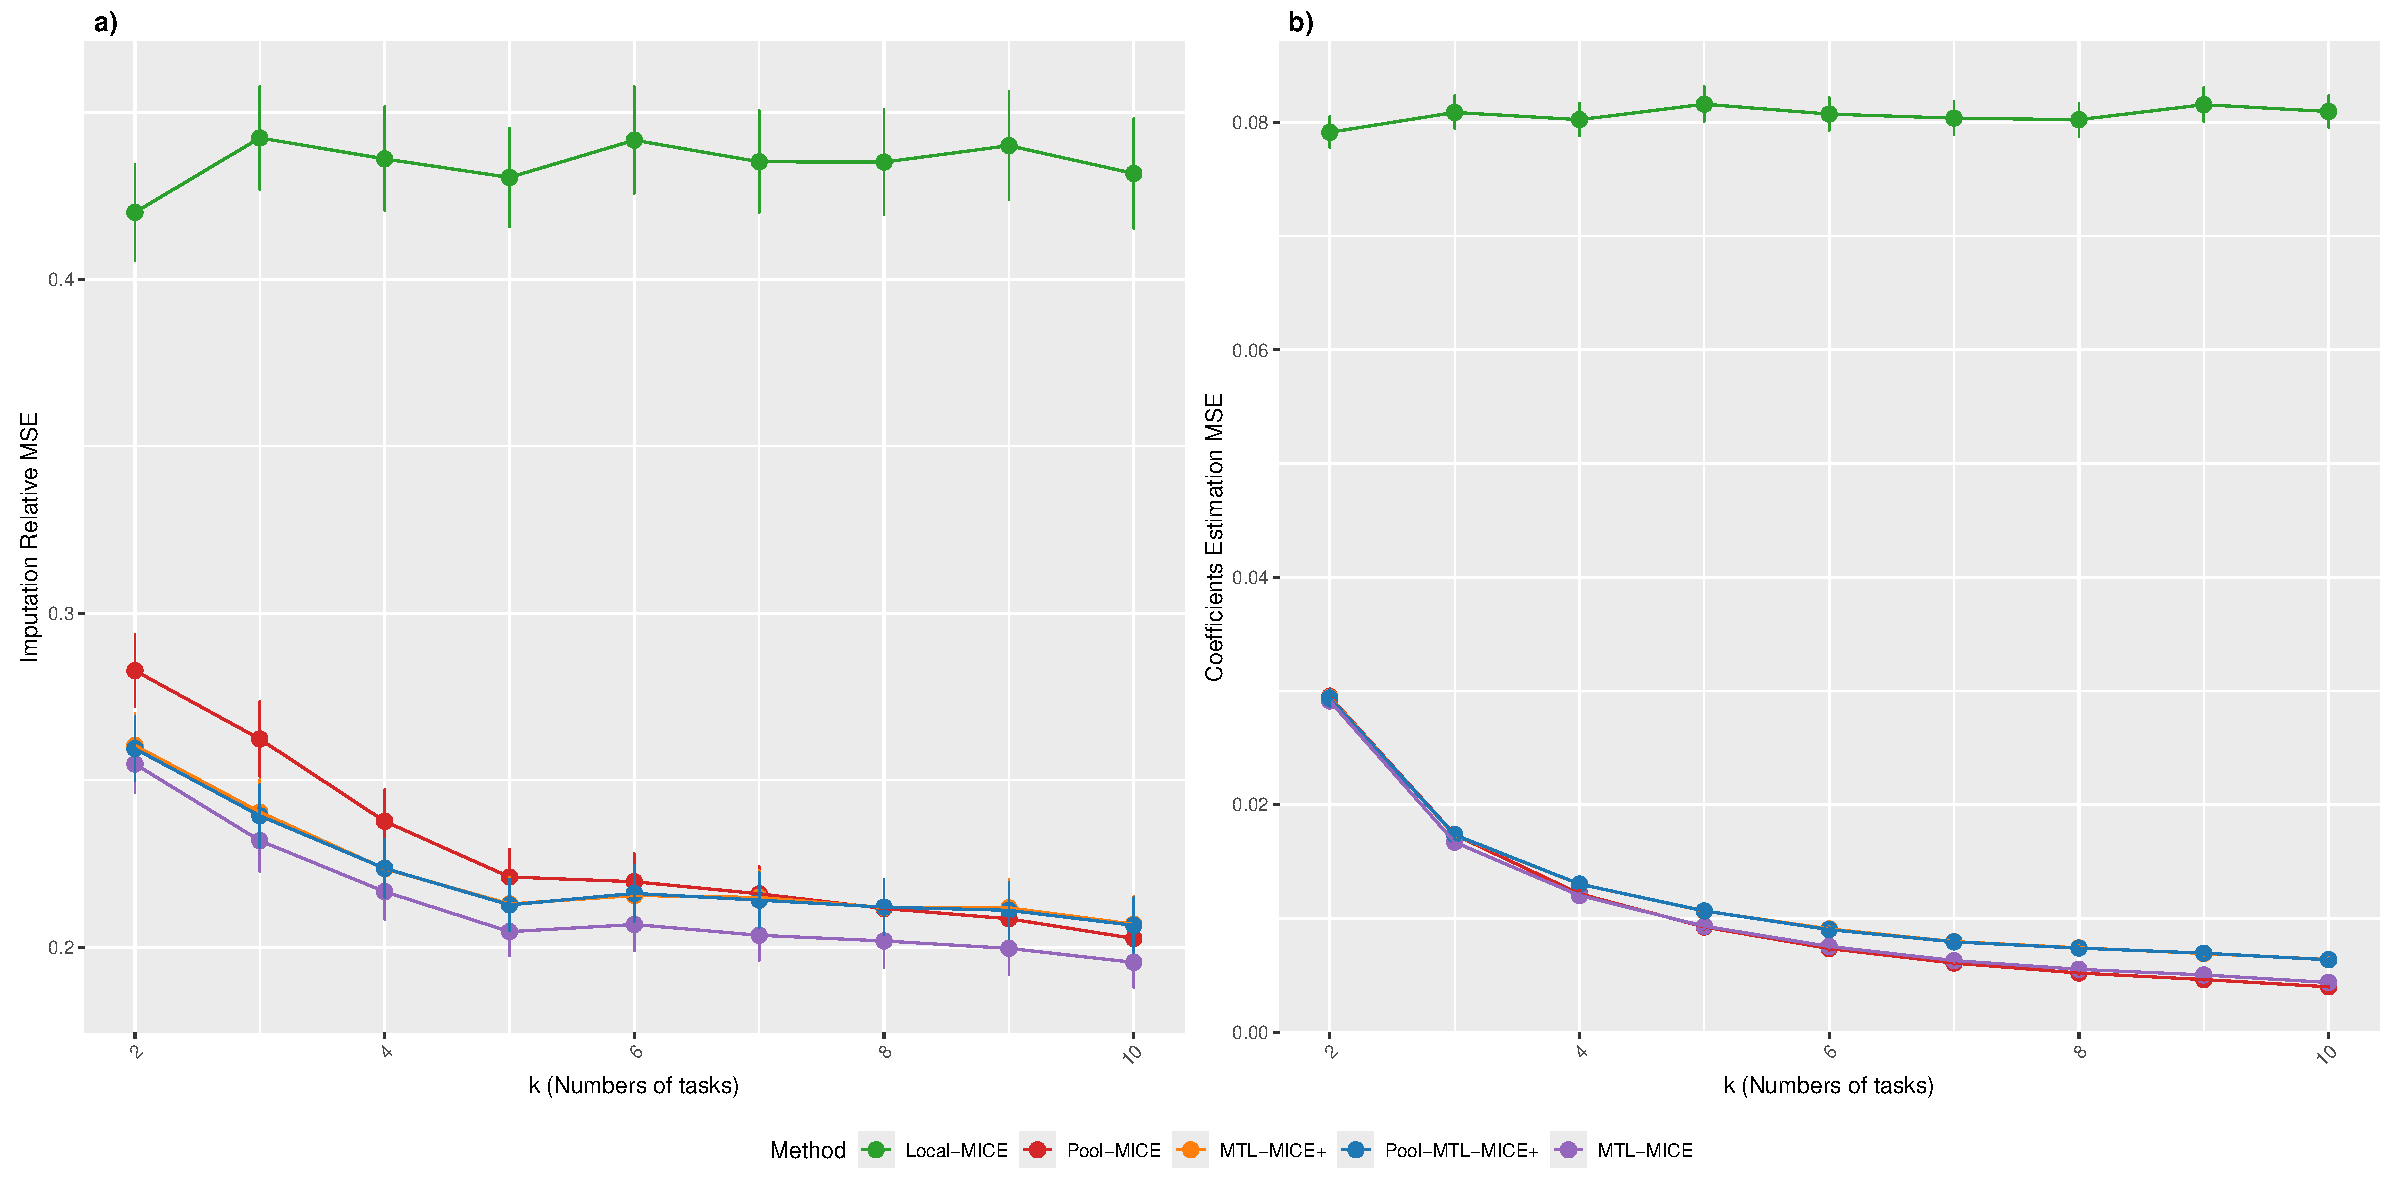
\includegraphics[width=1\linewidth]{plots/sim_ktrends_1se_continuous_rss_coeff.pdf}

\caption{$K$-trend simulation (varying the number of tasks).
We vary the number of available tasks $K\in\{2,3,\ldots,10\}$ with $n=100$, $p=150$, $v=15$, and one continuous incomplete variable.
Panel (a) reports continuous imputation relative MSE. Panel (b) reports coefficient MSE for the corresponding conditional model. Error bars show simulation uncertainty.}
\label{fig:ktrend_1x2}
\end{figure}

Figure~\ref{fig:htrend_1x2} summarizes the continuous-only $h$-trend experiment ($m=3$, $K=10$). Increasing $h$ increases across-task heterogeneity by perturbing task-specific coefficients away from the shared baseline, so transferability decreases and transfer-based methods gradually lose their advantage. When tasks are highly similar ($h\le 0.2$), pooled approaches and transfer-learning variants achieve substantially smaller $\mathrm{RelMSE}$ than Local-MICE, which reflects variance reduction from borrowing samples across tasks. In this range, MTL-MICE+ is typically best in both $\mathrm{RelMSE}$ and coefficient MSE, indicating that the correction step improves coefficient recovery even when mismatch is mild. As $h$ increases past about $0.3$, naive pooling degrades more quickly than detection-based methods and approaches the mean-imputation baseline ($\mathrm{RelMSE}\approx 1$) at the largest $h$ values. MTL-MICE and MTL-MICE+ degrade more smoothly, and remain competitive with Local-MICE across the sweep. Empirically, the largest and most consistent gains for MTL-MICE+ occur for $h\lesssim 0.3$, after which the benefit of transfer becomes small and source detection and correction mainly act to avoid the sharper losses seen under naive pooling.

\begin{figure}[t]
\centering
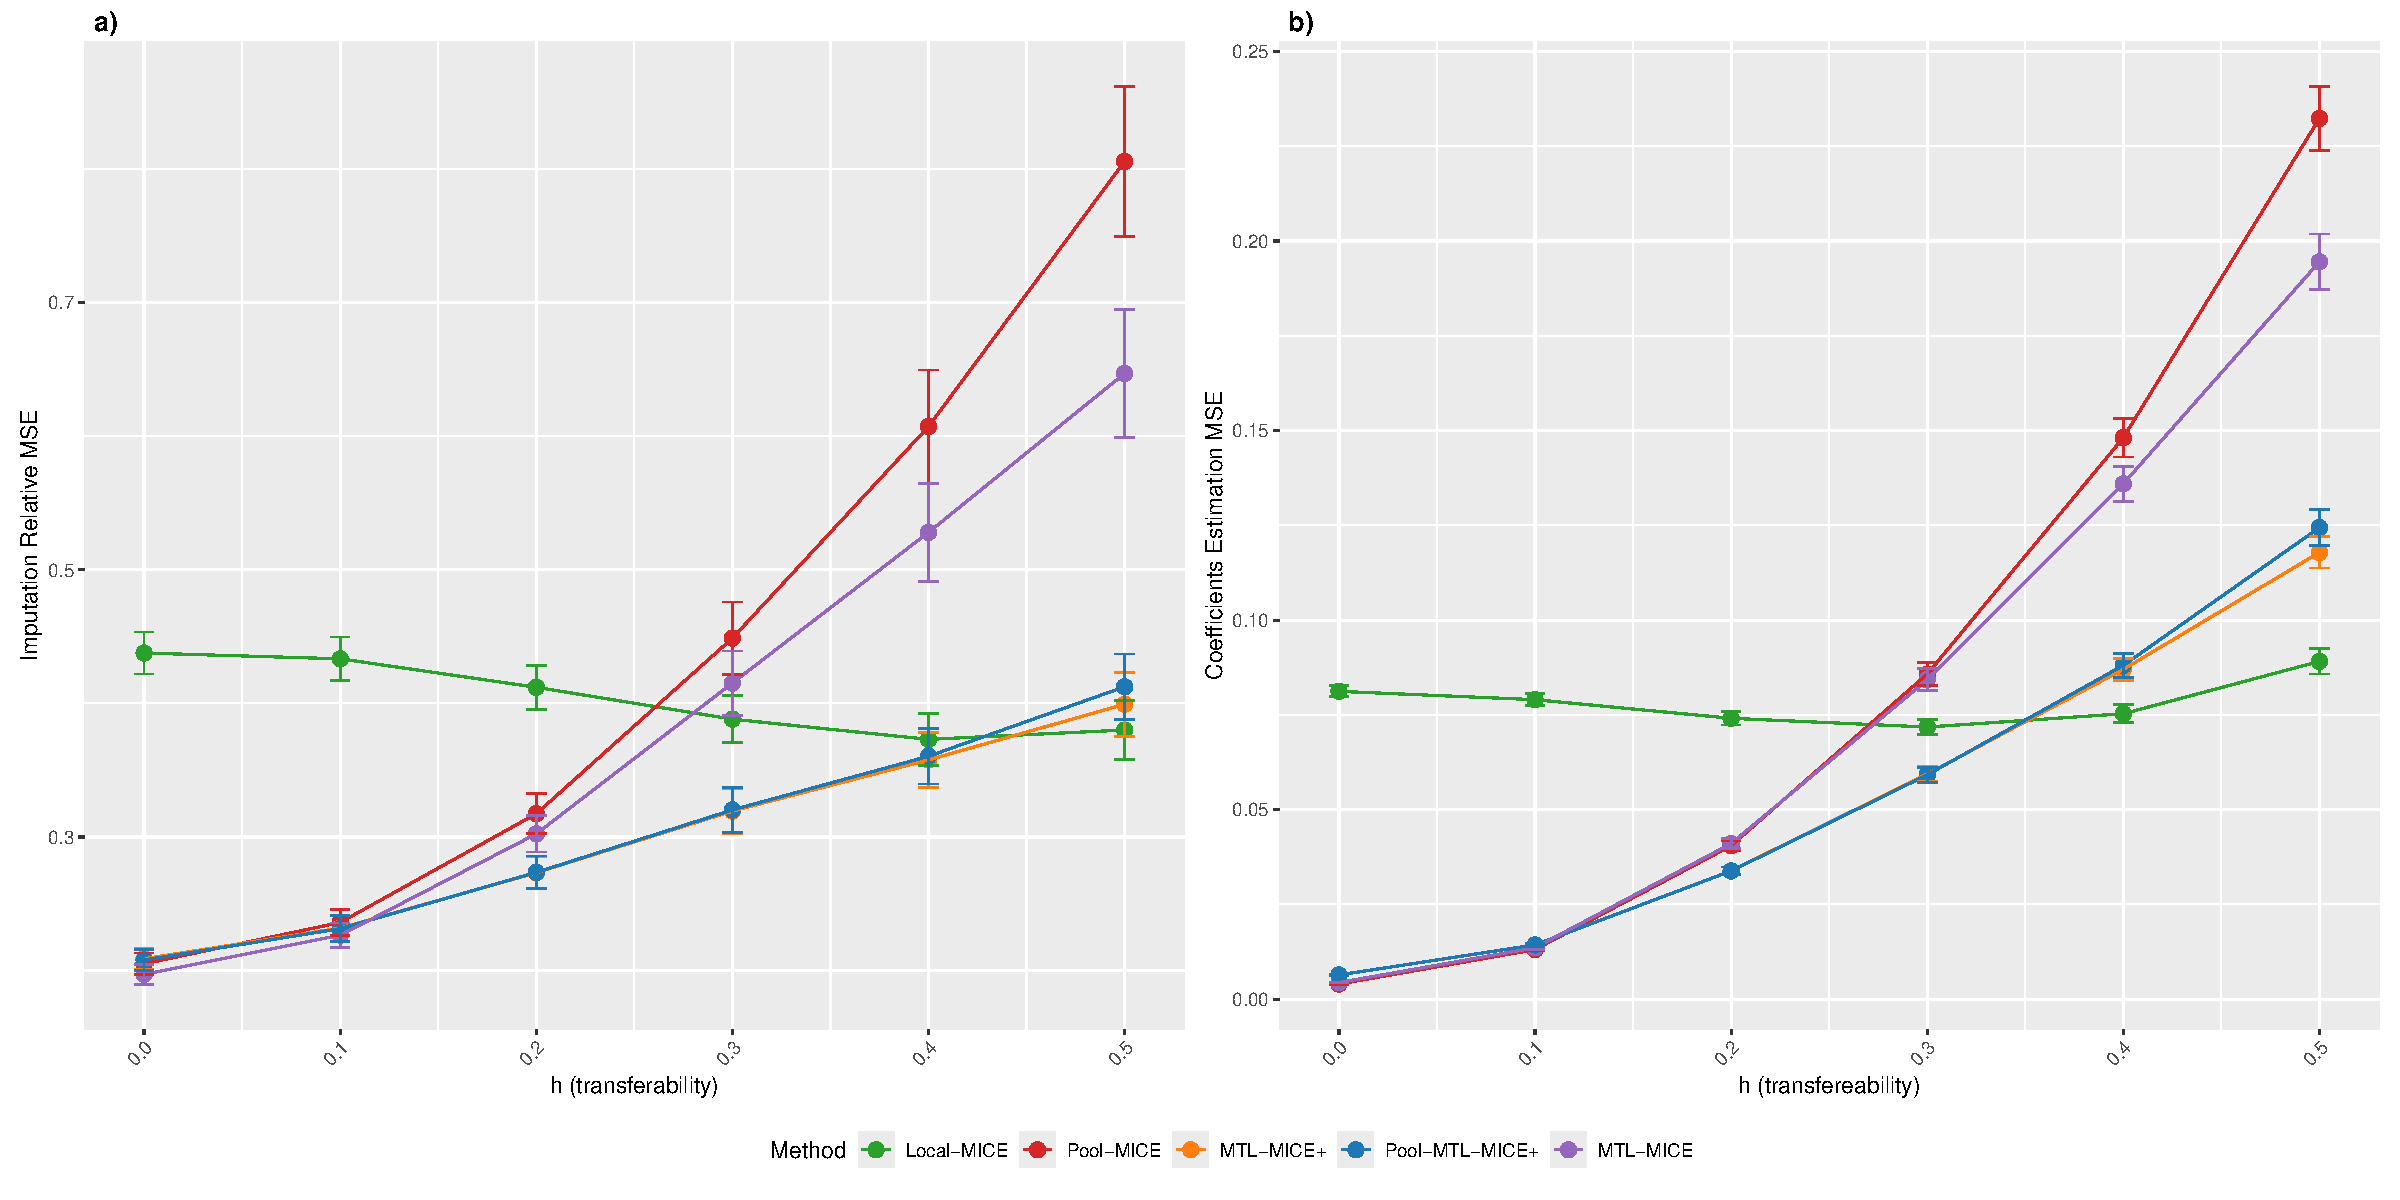
\includegraphics[width=1\linewidth]{plots/sim_htrends_1se_continuous_rss_coeff.pdf}

\caption{$h$-trend simulation (continuous-only incomplete variables).
We vary the transferability level $h\in\{0,0.1,\ldots,0.5\}$ with $n=100$, $p=150$, $v=15$, $K=10$, and $m=3$ continuous incomplete variables.
Panel (a) reports continuous imputation relative MSE.
Panel (b) reports coefficient MSE for the corresponding conditional models. Error bars show simulation uncertainty.}
\label{fig:htrend_1x2}
\end{figure}

In the mixed-type $h$-trend setting (two continuous and two binary incomplete variables; $K=10$), the effect of increasing $h$ depends on the variable type (Fig.~\ref{fig:htrend_mixed_2x2}). For the continuous outcomes, $\mathrm{RelMSE}$ is smallest for pooling-based methods and MTL-MICE+ when $h\le 0.2$, again reflecting variance reduction under strong transferability. As $h$ increases, negative transfer appears first for Pool-MICE: beyond about $h\approx 0.3$ its $\mathrm{RelMSE}$ rises rapidly and exceeds $1$ at the largest $h$ values, meaning it becomes worse than mean imputation. MTL-MICE+ remains comparatively stable as $h$ grows, and Pool-MTL-MICE+ also degrades more slowly than Pool-MICE, which is consistent with the target correction absorbing part of the mismatch. MTL-MICE, which uses the transferring-step coefficients without correction, degrades markedly once $h\gtrsim 0.3$, indicating that detection alone is not enough when the pooled coefficients are used directly for prediction. For the binary outcomes, accuracy decreases more gradually with $h$ for all transfer-based methods, and the spread across methods is smaller. MTL-MICE+ and Pool-MTL-MICE+ remain among the best across the full range of $h$, while Pool-MICE loses its early advantage and falls below them for $h\gtrsim 0.5$. The coefficient MSE panels match these patterns: coefficient error increases with $h$ for pooling-based estimators, but the increase is smaller when detection and correction are used.

\begin{figure}[t]
\centering
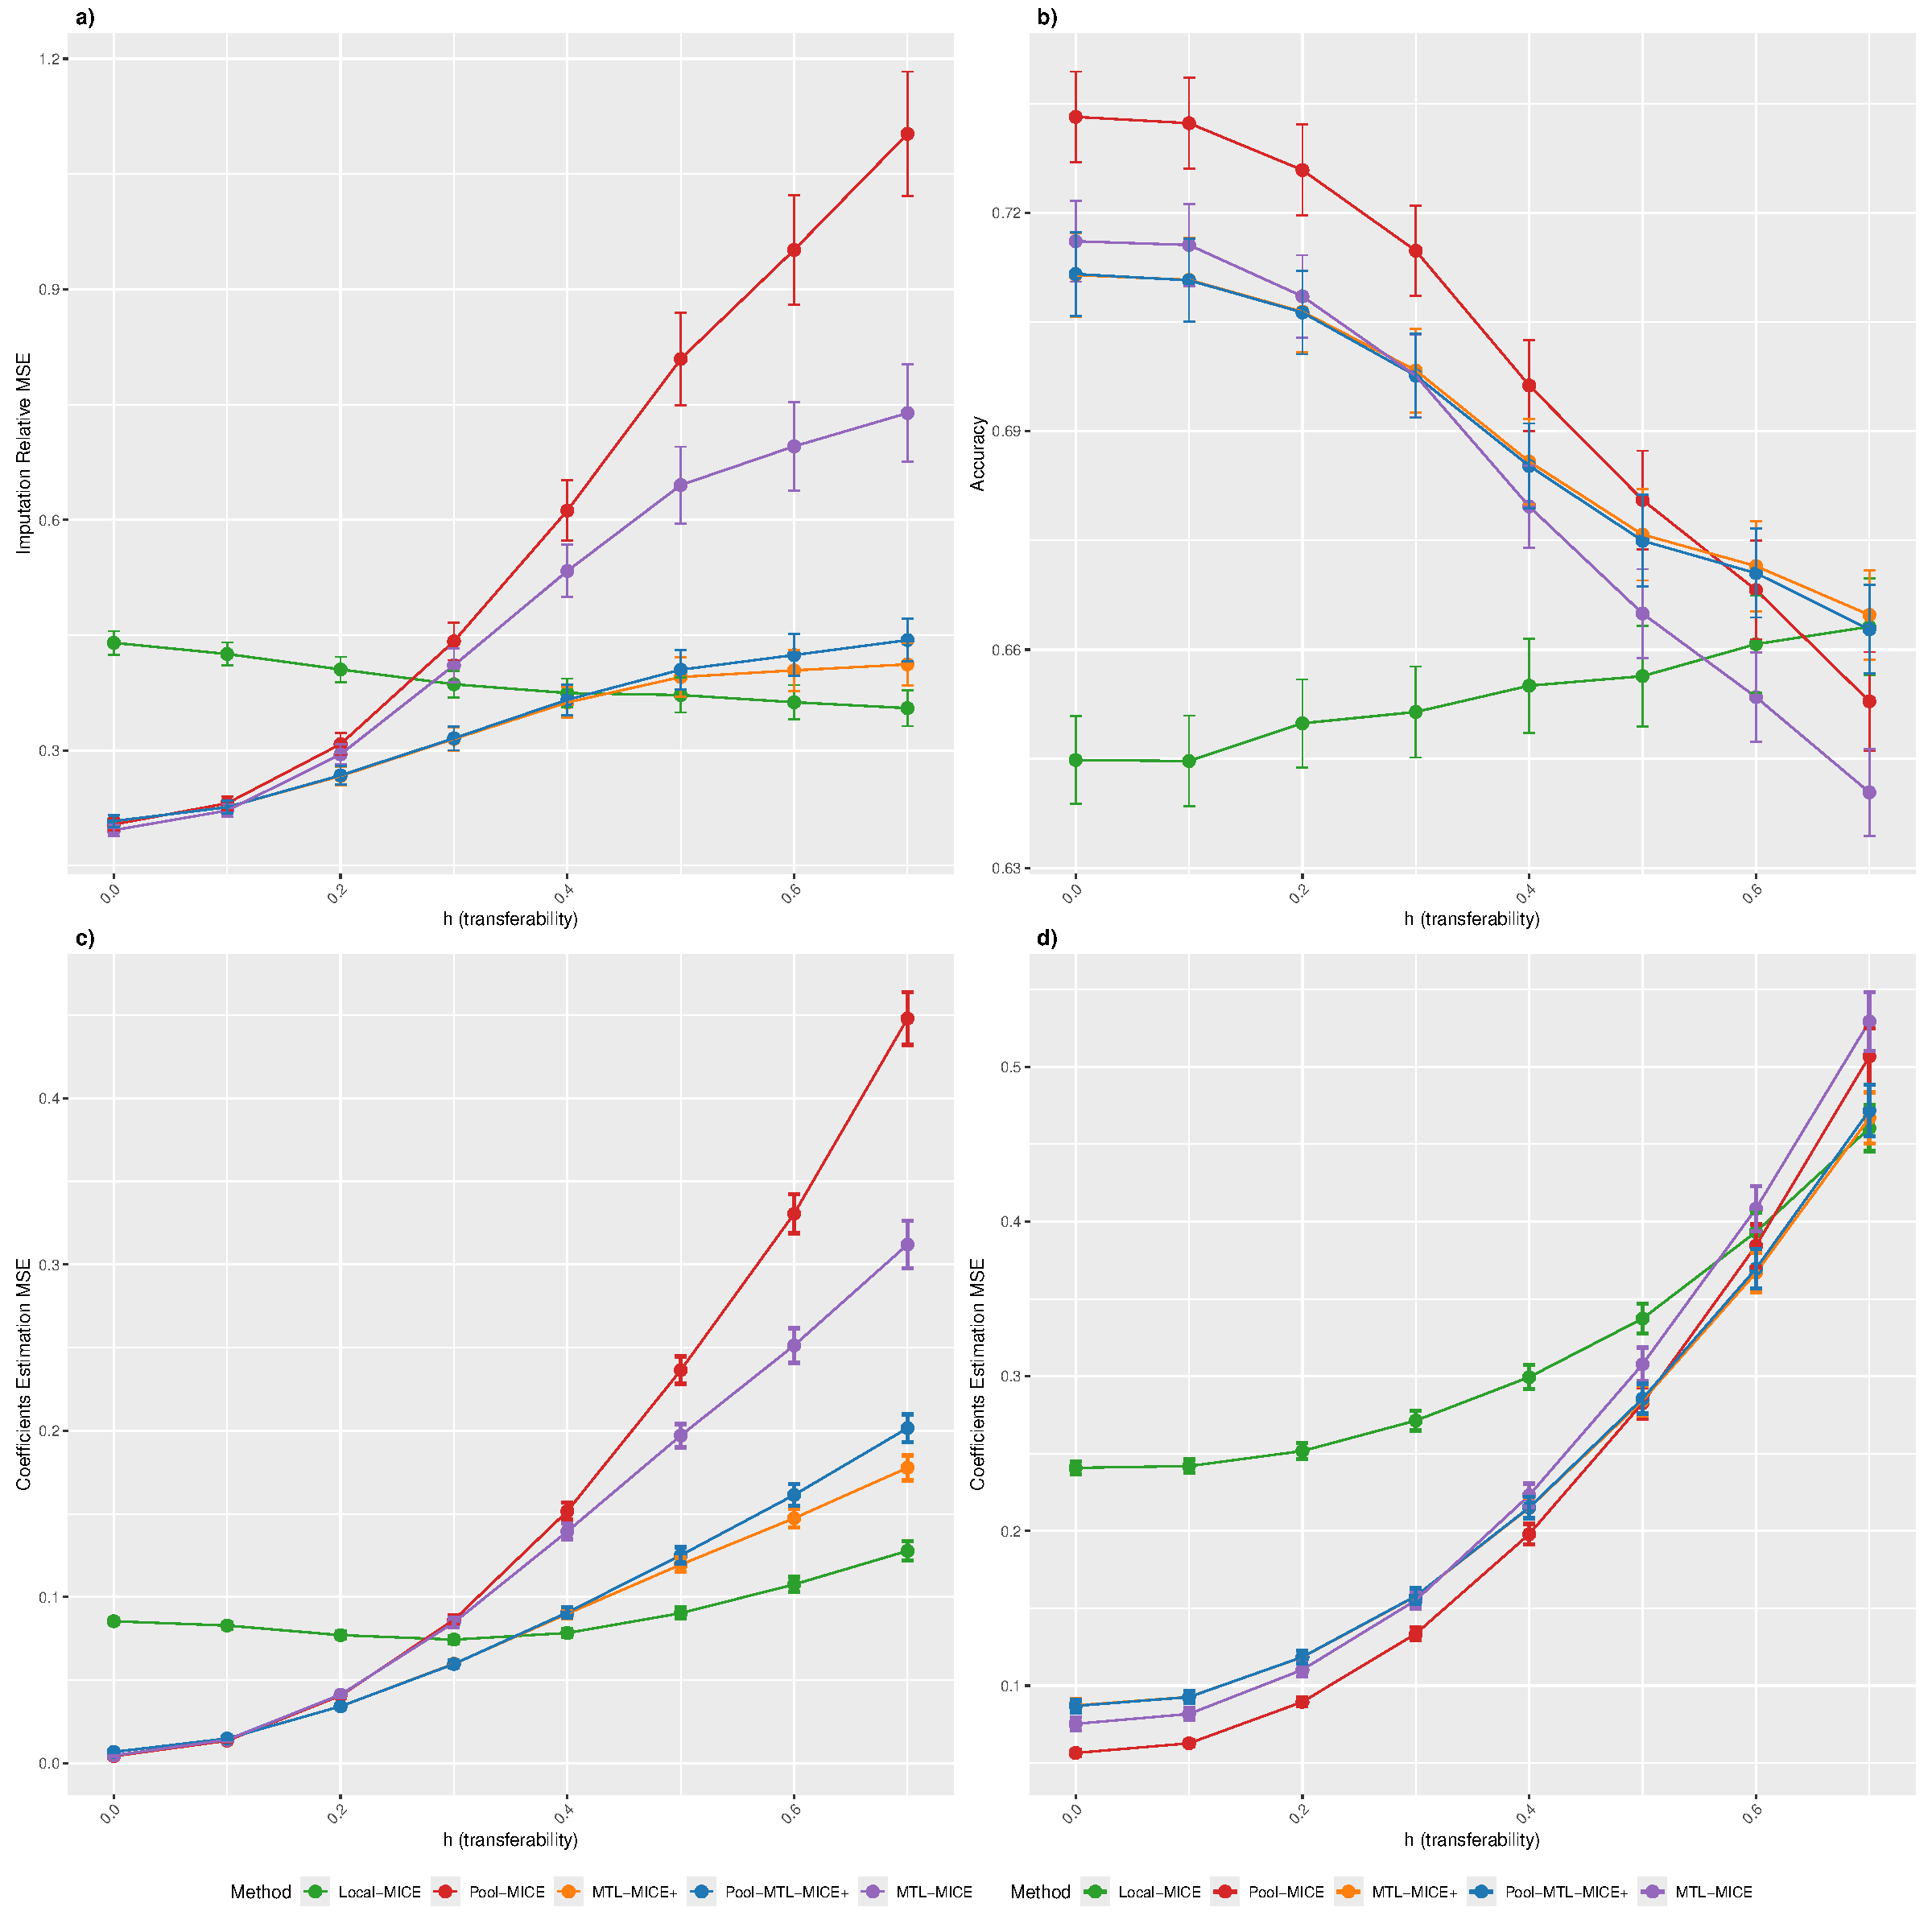
\includegraphics[width=0.9\linewidth]{plots/sim_htrends_mixed_combined_2x2_1se.pdf}

\caption{$h$-trend simulation with mixed missing-variable types.
Two continuous and two binary variables are incomplete ($n=100$, $p=150$, $v=15$, $K=10$), with transferability level
$h\in\{0,0.1,\ldots,0.7\}$ controlling cross-task similarity.
Panel (a) reports continuous imputation relative MSE. Panel (b) reports binary accuracy. Panels (c)–(d) report coefficient MSE for the corresponding conditional models. Error bars show simulation uncertainty.}
\label{fig:htrend_mixed_2x2}
\end{figure}

Figure~\ref{fig:htrend_cluster_2x2_cluster1} reports the clustered $h$-trend results (Cluster 1 only, since the two clusters are symmetric). Here $h$ controls within-cluster perturbations around cluster-specific baselines, with $\bm{B}^{(1)}_0=-2\cdot\bm{1}$ and $\bm{B}^{(2)}_0=+2\cdot\bm{1}$. Because the baseline coefficient magnitude is larger than in the mixed-type $h$-trend experiment (baseline $0.5$), the same absolute $h$ corresponds to a smaller relative perturbation, so the range $h\in[0,1.5]$ is needed to span mild to substantial mismatch in this setting. The main feature of this experiment is the cost of pooling across clusters with opposing baselines. Pool-MICE performs poorly for all $h$, with $\mathrm{RelMSE}$ close to $2$ and binary accuracy near chance, reflecting strong negative transfer from mixing tasks across clusters. Methods that use Trans-GLM detection largely avoid this failure mode by screening out cross-cluster sources. In this setting, detection is the primary safeguard: MTL-MICE achieves the smallest $\mathrm{RelMSE}$ over most of the $h$ range and remains competitive with or better than Local-MICE even at $h=1.5$, while maintaining the highest binary accuracy as $h$ increases. The correction step has a different role. Comparing Pool-MICE to Pool-MTL-MICE+ shows that correction substantially reduces the damage of indiscriminate pooling, even without detection. After detection has already selected mostly within-cluster sources, the added correction can have limited benefit and may increase variance in finite samples, so MTL-MICE+ is not uniformly better than MTL-MICE in this clustered regime. This behavior is consistent with the correction step trading bias reduction for variance, with the balance depending on how homogeneous the detected source set is.

\begin{figure}[t]
\centering
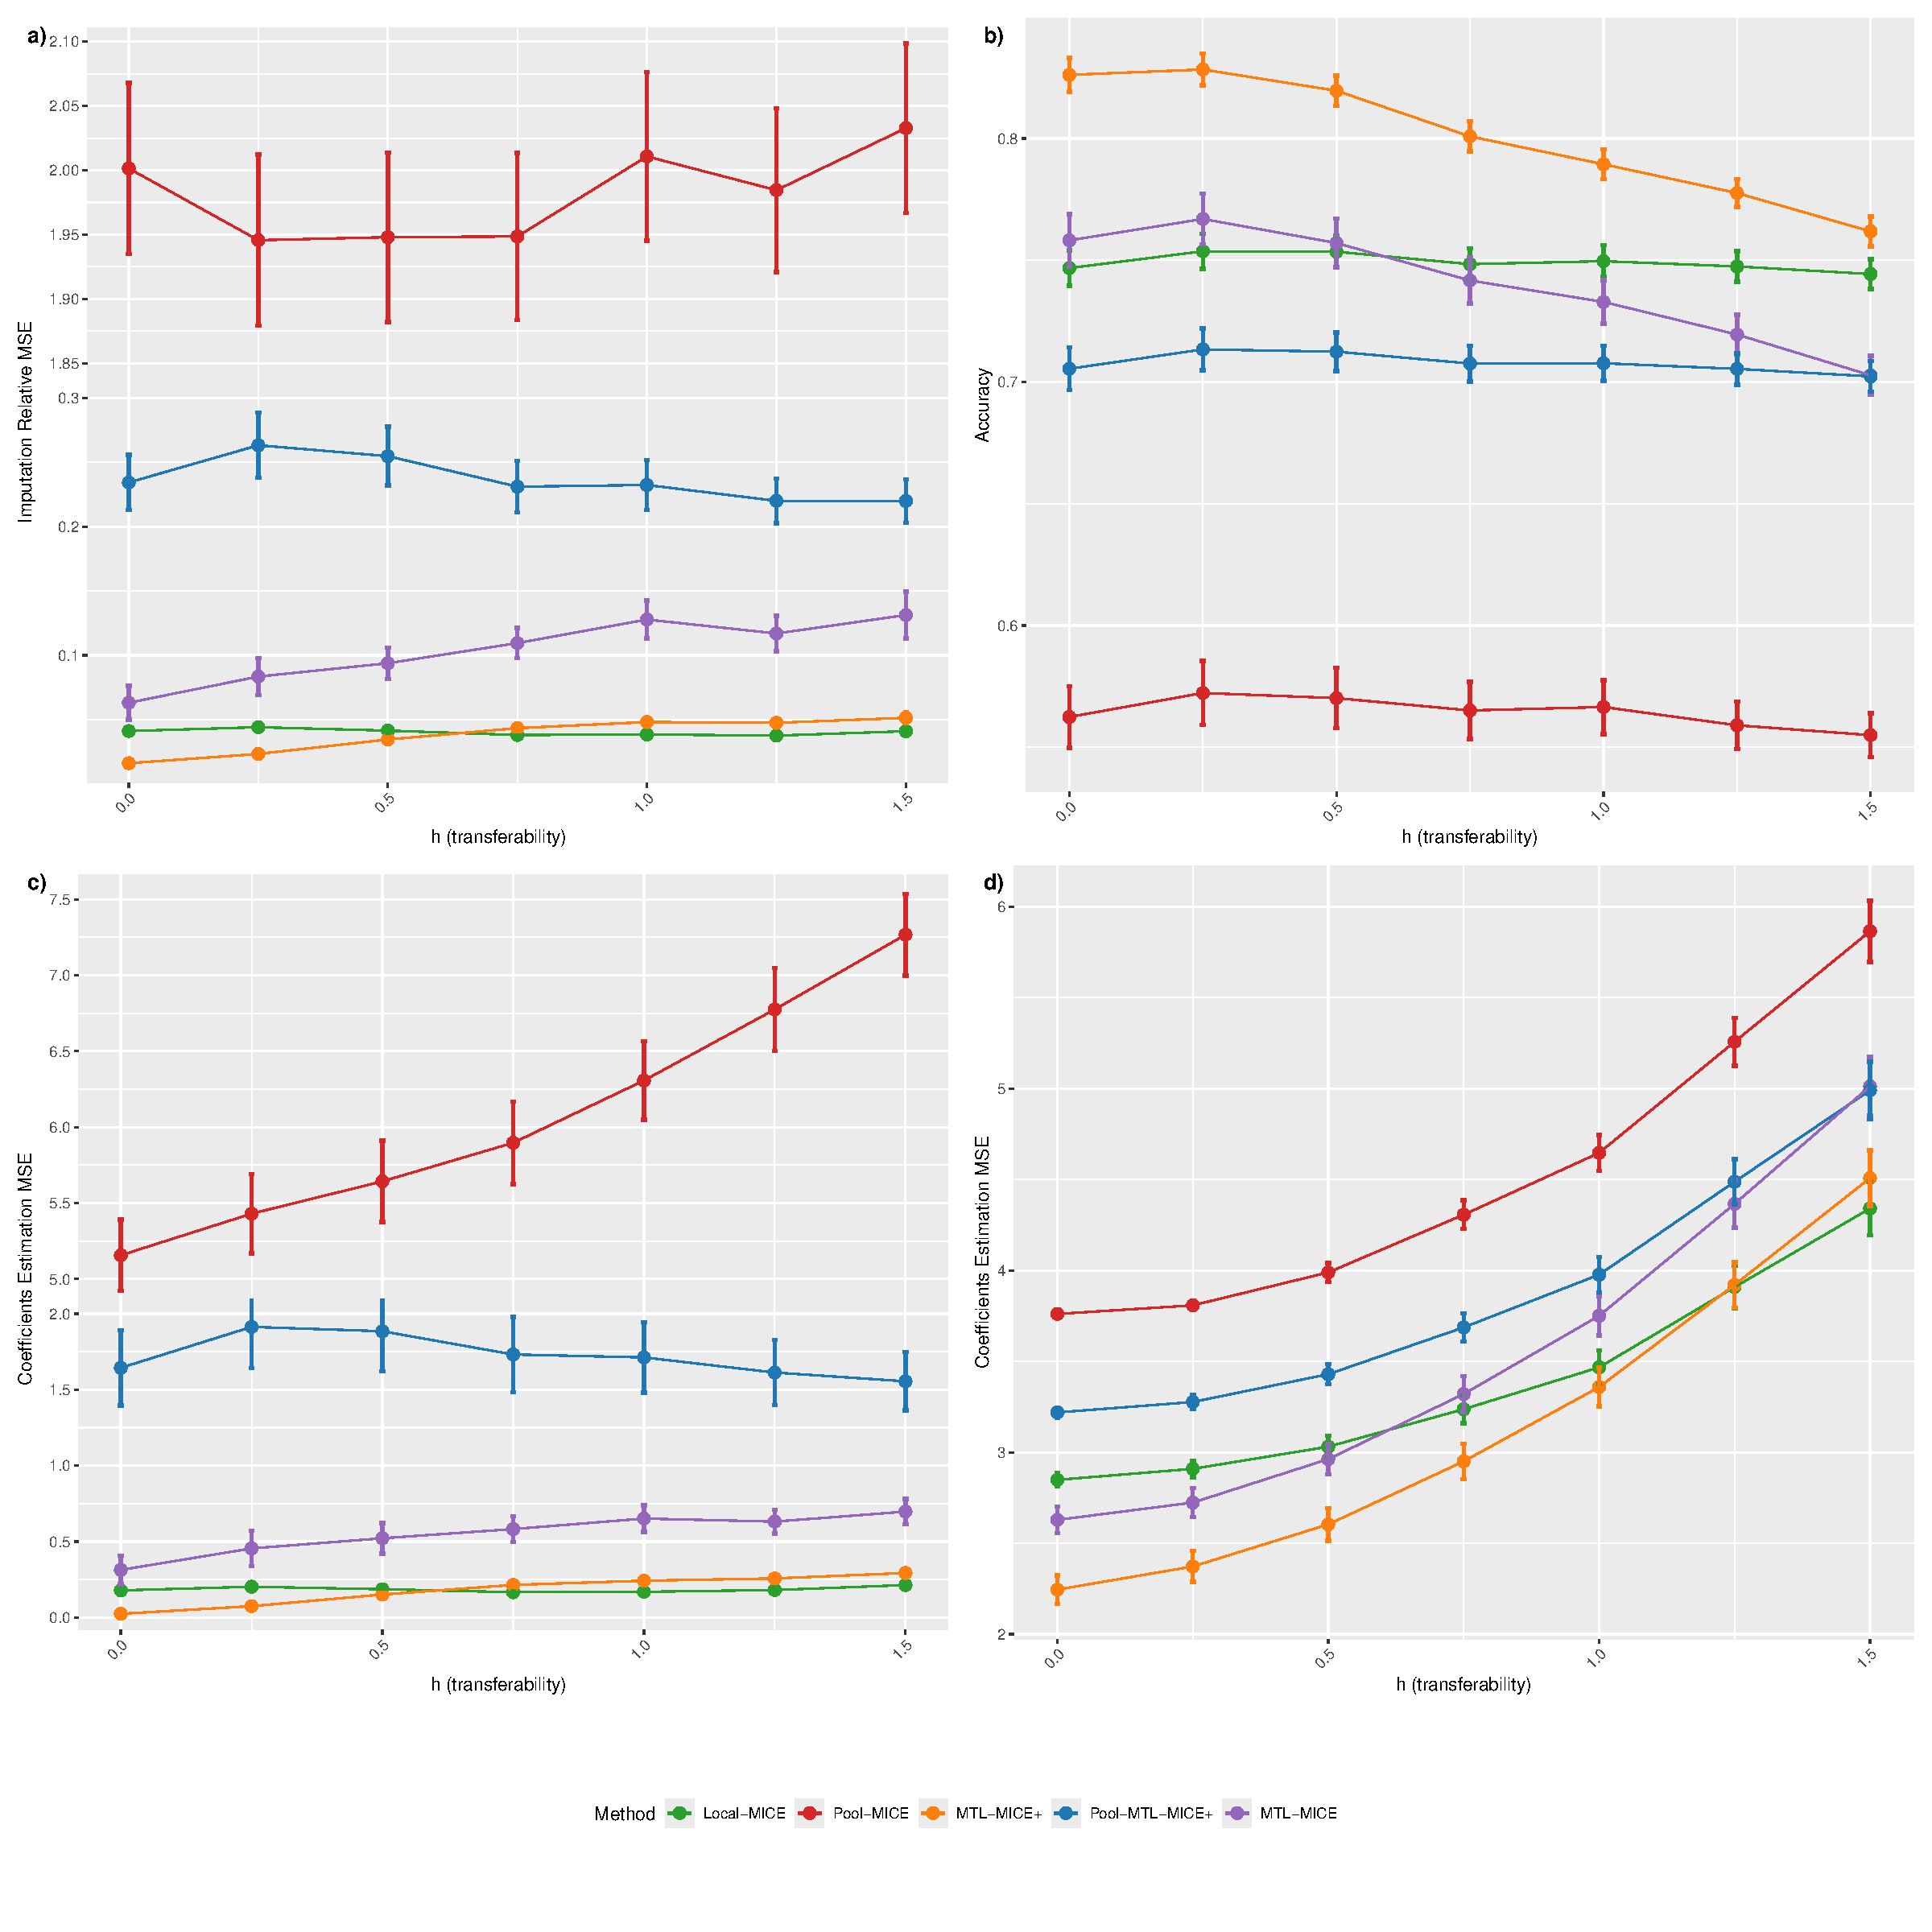
\includegraphics[width=0.9\linewidth]{plots/sim_htrends_cluster_combined_2x2_1se_1.pdf}

\caption{$h$-trend simulation with clustered tasks (Cluster 1 shown).
Panels (a)–(b) summarize imputation performance as transferability decreases (larger $h$ implies weaker similarity within cluster), while panels (c)–(d) report coefficient recovery for the corresponding conditional models. Error bars show simulation uncertainty.}
\label{fig:htrend_cluster_2x2_cluster1}
\end{figure}

In the outlier experiment (Fig.~\ref{fig:htrend_outlier_2x2_tasks1to9}), tasks 1--9 share the baseline $\bm{B}_0=-2\cdot\bm{1}$ and task 10 is generated from $\bm{C}_0=+2\cdot\bm{1}$. We report performance on tasks 1--9 to isolate the effect of a single non-transferable source. As in the clustered case, the baseline magnitude implies that larger $h$ values correspond to moderate relative perturbations compared to the mixed-type setting. For continuous imputation, Pool-MICE is much worse than all other methods across the full $h$ range, indicating that including the outlier in a pooled fit produces large negative transfer even when tasks 1--9 are mutually similar. Pool-MTL-MICE+ reduces this damage, but remains worse than the detection-based methods, which is consistent with correction alone being insufficient when an opposing outlier is always included. Trans-GLM detection makes the transfer-based methods robust by screening out the outlier. Within the detected-transfer regime, the correction step becomes more important as $h$ increases: MTL-MICE degrades quickly once $h\gtrsim 0.5$, while MTL-MICE+ remains close to the best curve and avoids the large losses seen under pooling. For binary imputation, MTL-MICE+ has the highest accuracy across $h$, with MTL-MICE close behind, and both remain above Local-MICE even at $h=1.5$. The coefficient MSE panels support the same interpretation, showing that detection prevents the large coefficient errors induced by pooling with the outlier, while correction helps stabilize coefficient estimation as within-group transferability weakens.

\begin{figure}[t]
\centering
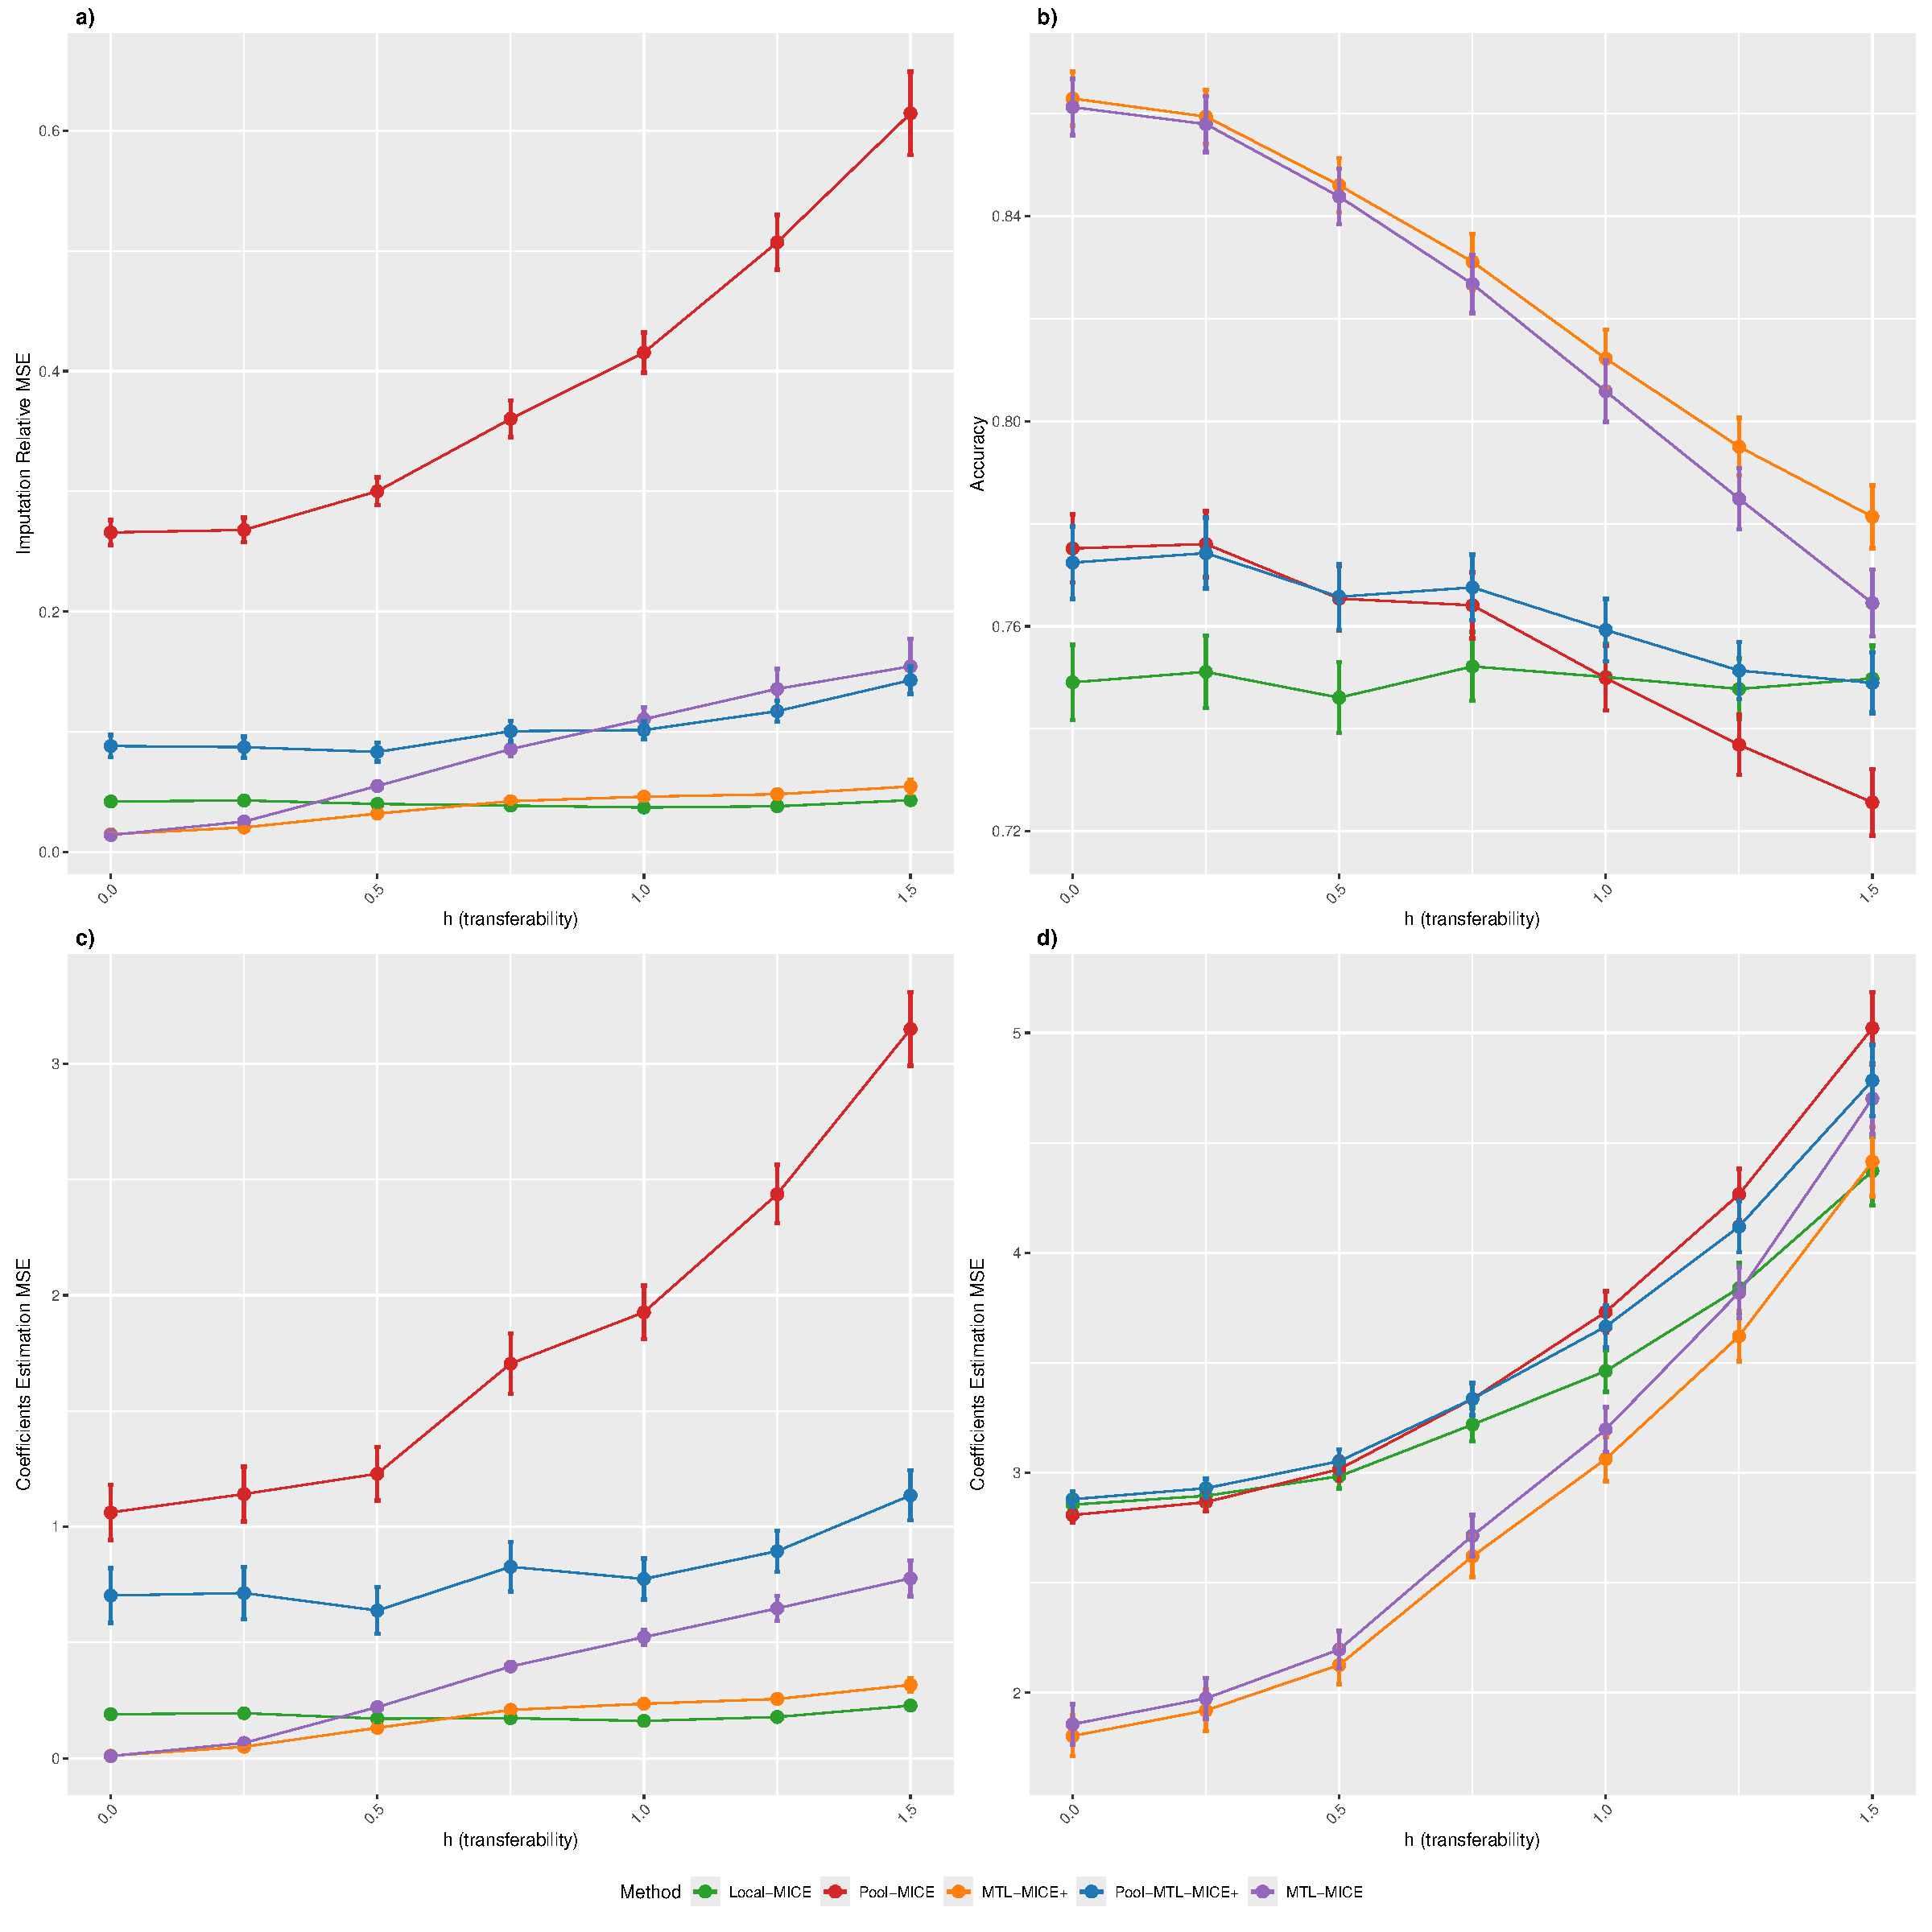
\includegraphics[width=0.9\linewidth]{plots/sim_htrends_outlier_combined_2x2_1se.pdf}

\caption{$h$-trend simulation with an outlier task (tasks 1--9 shown).Task $10$ is an outlier generated from an opposing baseline (negative transfer if pooled).
Panels (a)–(b) summarize imputation performance as within-group transferability decreases,
while panels (c)–(d) report coefficient recovery for the corresponding conditional models, where (c) is for continuous and (d) is for binary. Error bars show simulation uncertainty.}
\label{fig:htrend_outlier_2x2_tasks1to9}
\end{figure}

\section{Real Data Analysis}
\label{sec:realdata}

We evaluate the proposed multi-task imputation methods on county-level data from the 2020 U.S.\ presidential election. County-level two-party outcomes (Democratic versus Republican winner) are obtained from \url{https://github.com/tonmcg/US_County_Level_Election_Results_08-20}. County-level social and demographic covariates, including population and race proportions, are merged from \url{https://www.kaggle.com/benhamner/2016-us-election}. We merge the datasets using county identifiers and restrict attention to states with county-equivalent units. Alaska is excluded because it does not have counties in the same sense as other states, and Washington, D.C.\ is excluded because it is not a state-level unit.

We treat each state as a task and counties as samples within the task. For state $k$, we construct a data matrix $\bm{X}^{(k)}\in\mathbb{R}^{n_k\times p}$, where $n_k$ is the number of counties in the state and $p$ is the number of variables after preprocessing. In each experiment, one state is treated as the target task and the remaining states are candidate sources. Transfer is applied within each chained-equation update, so the transferring set can differ by target state and by the variable being imputed.

To focus on states that are not overwhelmingly dominated by either party and that have enough counties for stable evaluation, we select target states for which the proportion of counties voting Democratic in 2020 lies in $[10\%,90\%]$ and the state contains at least 75 counties. This yields eight target states: Arkansas (AR), Georgia (GA), Illinois (IL), Michigan (MI), Minnesota (MN), Mississippi (MS), North Carolina (NC), and Virginia (VA).

We evaluate imputation accuracy on two county-level covariates with different data types. The continuous outcome is median housing value. The binary outcome is an indicator for multi-unit housing at least 10\%, where the cutoff is chosen based on the empirical distribution to avoid extreme class imbalance. All remaining covariates are treated as predictors in the conditional models.

For each target state, we introduce missingness under a missing-at-random mechanism by masking entries of the evaluation variables with probabilities that depend on other observed county-level covariates through a logistic model. We consider missing rates $\rho\in\{10\%,20\%,30\%,40\%,50\%\}$, and for each $\rho$ we repeat the masking 100 times with independent missingness masks. Each repetition uses the same number of imputations $M$ and MICE iterations $T$ across methods, and we average results across repetitions. Performance is summarized using the same metrics as in the simulation study: for the continuous variable we report imputation relative MSE against mean imputation within the target state, and for the binary variable we report accuracy on masked cells.

\subsection{Real Data Analysis Results}
\label{subsec:rda_results}

Figure~\ref{fig:rda_us_election} summarizes imputation performance on the 2020 county-level election dataset, with states treated as tasks and counties treated as samples within each task. The target states are AR ($n=75$), GA ($n=159$), IL ($n=102$), MI ($n=83$), MN ($n=87$), MS ($n=82$), NC ($n=100$), and VA ($n=133$). For each target state, missingness is introduced under MAR at rates $\rho\in\{10\%,20\%,30\%,40\%,50\%\}$, and results are averaged over 100 independent missingness masks. The continuous evaluation variable is median housing value and the binary evaluation variable is the indicator for multi-unit housing at least 10\%.

Averaged across the target states (Fig.~\ref{fig:rda_us_election}), all methods show degradation as the missingness rate increases, but the degree and order depend on the type of variable. FOverall, MTL-MICE+ is the best method for the continuous outcome at all missing rates below $1-R^2_{\mathrm{out}}$, and Pool-MTL-MICE+ is the second-best method. Both are well below the performance of Local-MICE and Pool-MICE. The gap between MTL-MICE+ and the other methods increases as the missingness rate increases, which makes sense since the value of transfer is greatest when the effective sample size in the target task is small. Pool-MICE is the worst method for the continuous outcome at all but the highest missingness rates, suggesting that this method is affected by cross-state variation in the conditional relationship between the median housing value and the socio-demographic predictors. The average performance over the target states confirms two findings from the simulation study. First, naive pooling can introduce negative transfer for continuous outcomes. Second, when transfer is used, the correction step in MTL-MICE+ stabilizes the conditional model and improves imputation accuracy across a range of missingness rates.

For the binary outcome, the methods differ less on average (Fig.~\ref{fig:rda_us_election}b). For all methods, accuracy is negatively related to missingness, though MTL-MICE+ and Pool-MTL-MICE+ attain the highest or second-highest accuracy for moderate and high missingness rates. For low missingness, Local-MICE is competitive, though its accuracy drops more precipitously as missingness increases, as expected under the logistic model with only the target variable, which is losing information as the number of observed outcomes diminishes. For Pool-MICE, accuracy is more variable as missingness increases, consistent with cross-state heterogeneity. MTL-MICE, using the transferring step coefficients without the correction term, performs least well for the binary outcome across all missingness rates. This suggests that for this binary variable, using pooled coefficients can be problematic when cross-state differences in the logistic relationship are present, and the correction term helps to reduce this sensitivity to cross-state variation.

\begin{figure}[t]
\centering
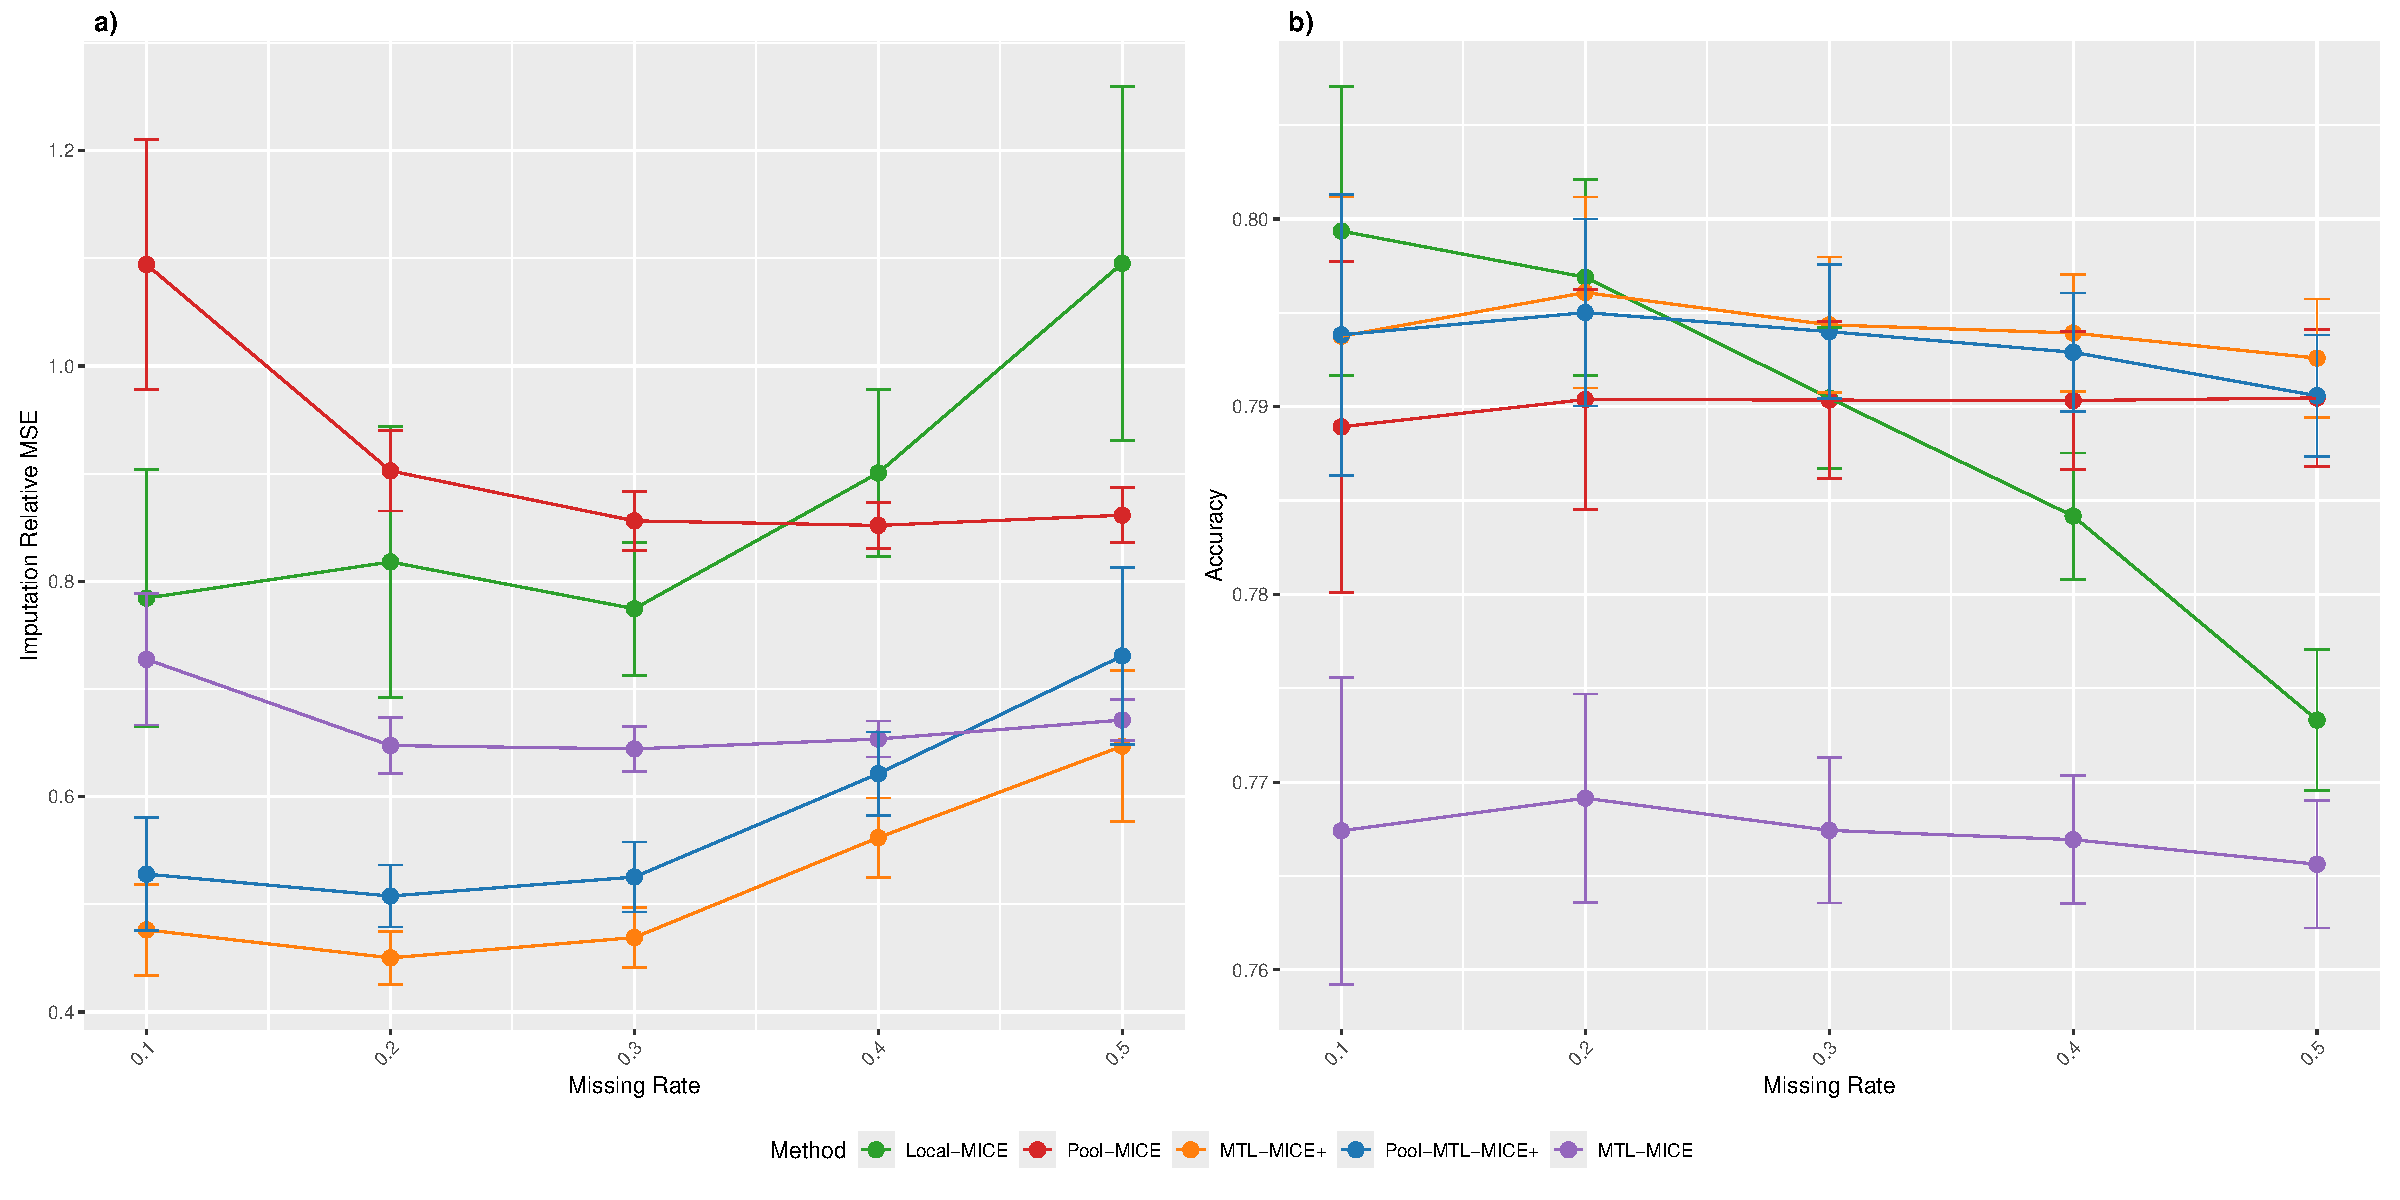
\includegraphics[width=1\linewidth]{plots/rda_uselection_combined_plot.pdf}

\caption{Real-data analysis: county-level 2020 U.S.\ presidential election data. For the continuous variable (median housing value), we report imputation relative MSE. For the binary variable (multi-unit housing $\ge 10\%$), we report accuracy on masked cells (larger is better). Panels (a) is the imputation relative MSE averaged over target states, while
(b) is the accuracy on masked cells averaged over target states.}
\label{fig:rda_us_election}
\end{figure}

State-level results (Fig.~\ref{fig:rda_cont_bystate},\ref{fig:rda_bin_bystate}) indicate that transfer benefits differ for different target states, and this can be explained by both the number of samples in a target state and how heterogeneous the target-state’s conditional model appears in comparison to the candidate sources. In terms of the continuous variable, Minnesota(MN) is a case where Local MICE deteriorates very fast as the amount of missing data increases, while MTL-MICE+ and Pool-MTL-MICE+ remain much more stable. This is because the target-only model is not powerful enough as the number of observed counties decreases, while transfer helps more in this case. Michigan(MI) results in large separation overall, with Pool MICE performing particularly badly and transfer methods with correction having the lowest errors. Virginia(VA) results in relatively small differences in overall errors for different methods, especially at lower levels of missing data, which suggests that the target-only model’s conditionality is already quite stable given the number of counties and available predictors. Georgia(GA) results in smaller benefits from transfer for lower to moderate levels of missing data, while transfer is still beneficial for higher levels of missing data because it has the largest number of counties among all target states.

For the binary outcome, the state-specific plots show a different pattern. In this case, the gap between the transfer methods and the Local-MICE model appears smaller, with some states showing little difference between methods. In states where the binary outcome is easier to predict based on the covariates (for example, states where the distribution of the multi-unit indicator lines up well with urbanization-related predictors), the pooling-based methods are still competitive. In Michigan (MI) and Mississippi (MS), there appears to be strong performance of the pooling-based methods, while in Minnesota (MN) and North Carolina (NC), there appears to be clear improvement of the methods incorporating the correction step. This pattern supports the notion that the binary outcome decision boundary is more transferable across states than the continuous price level, but still benefits from correction when the target distribution has a different structure, particularly at higher missingness levels.

To investigate which states are selected as transferable sources and how this differs across variables, we summarize the Trans-GLM source detection output as directed transferability networks (Fig.~\ref{fig:rda_transfer_con} and Fig.~\ref{fig:rda_transfer_bin}). For each target state $k\in\{\mathrm{AR,GA,IL,MI,MN,MS,NC,VA}\}$ and each evaluation variable, we run Trans-GLM on the target complete cases and obtain an estimated transferring set $\widehat{\mathcal{A}}^{(k)}$ of source states. We repeat this procedure across $R$ independent MAR masks and missing-rate settings, and define the transfer frequency for an ordered pair $(\ell\rightarrow k)$ as
\(\mathrm{freq}(\ell\rightarrow k)
=\frac{1}{R}\sum_{r=1}^{R}\mathbb{I}\{\ell\in\widehat{\mathcal{A}}^{(k)}(r)\}.\)
We then visualize the 10 directed state pairs with the largest transfer frequencies. Nodes represent states, with target states shown in orange and source states shown in blue. A directed edge $\ell\rightarrow k$ indicates that $\ell$ is among the most consistently selected sources for target $k$ for that variable.

The continuous-variable network (Fig.~\ref{fig:rda_transfer_con}) shows a clear regional structure. The dense set of high-frequency edges is concentrated among states that are either geographically proximate to each other or have similar socio-economic composition at the county level. This is because the median value of housing is likely to be related to the regional housing markets, which depend on the regional labor markets, regional cost of living, and regional constraints on the supply of housing that can be bought and sold. Therefore, the conditional relationship between the housing value and the set of demographic and housing-stock related covariates is best transferred among states that have similar regional economic and geographic contexts. The qualitative explanation for the poor performance of naive methods on the continuous outcome is that the Pool-MICE method implicitly assumes the existence of the same conditional relationship across all states, when in fact the Trans-GLM method is selecting a subset of sources that is likely to be compatible with the target state.

The binary-variable network (Fig.~\ref{fig:rda_transfer_bin}) is more diffuse, with more long-range edges between non-adjacent states. This is consistent with the interpretation of the binary result as an indicator of housing stock density and urbanization. After adjusting for covariates such as population and racial proportions, the relationship between the predictors and the presence of substantial multi-unit housing in the county has the potential to generalize over all states with similar compositions of urban, suburban, and rural counties, even when the states are not geographically adjacent. Therefore, the network has more cross-region transfer links than the continuous network. This is consistent with the results for the binary accuracy model having less variability across methods because the binary conditional model has more potential for generalized results over the states than the continuous price level model, although the correction step provides benefits in the presence of high missing data rates and target-specific structure.

Overall, the results with the real data confirm the findings with the simulated data. The naive pooling method is least robust when the tasks have different conditional structures, and this is most obvious with the continuous outcome variable. The source detection and correction methods offer a way to leverage information across tasks while limiting negative transfer. The transferability networks provide an extra level of interpretation because they show which state pairs consistently met the detection criterion and indicate that the transferability depends on the variable type; the housing value transfer links depend on regional economic similarities, and the multi-unit indicator transfer links depend on similarities in county typologies.


\begin{figure*}[t]
\centering

\begin{subfigure}[t]{0.6\linewidth}
    \centering
    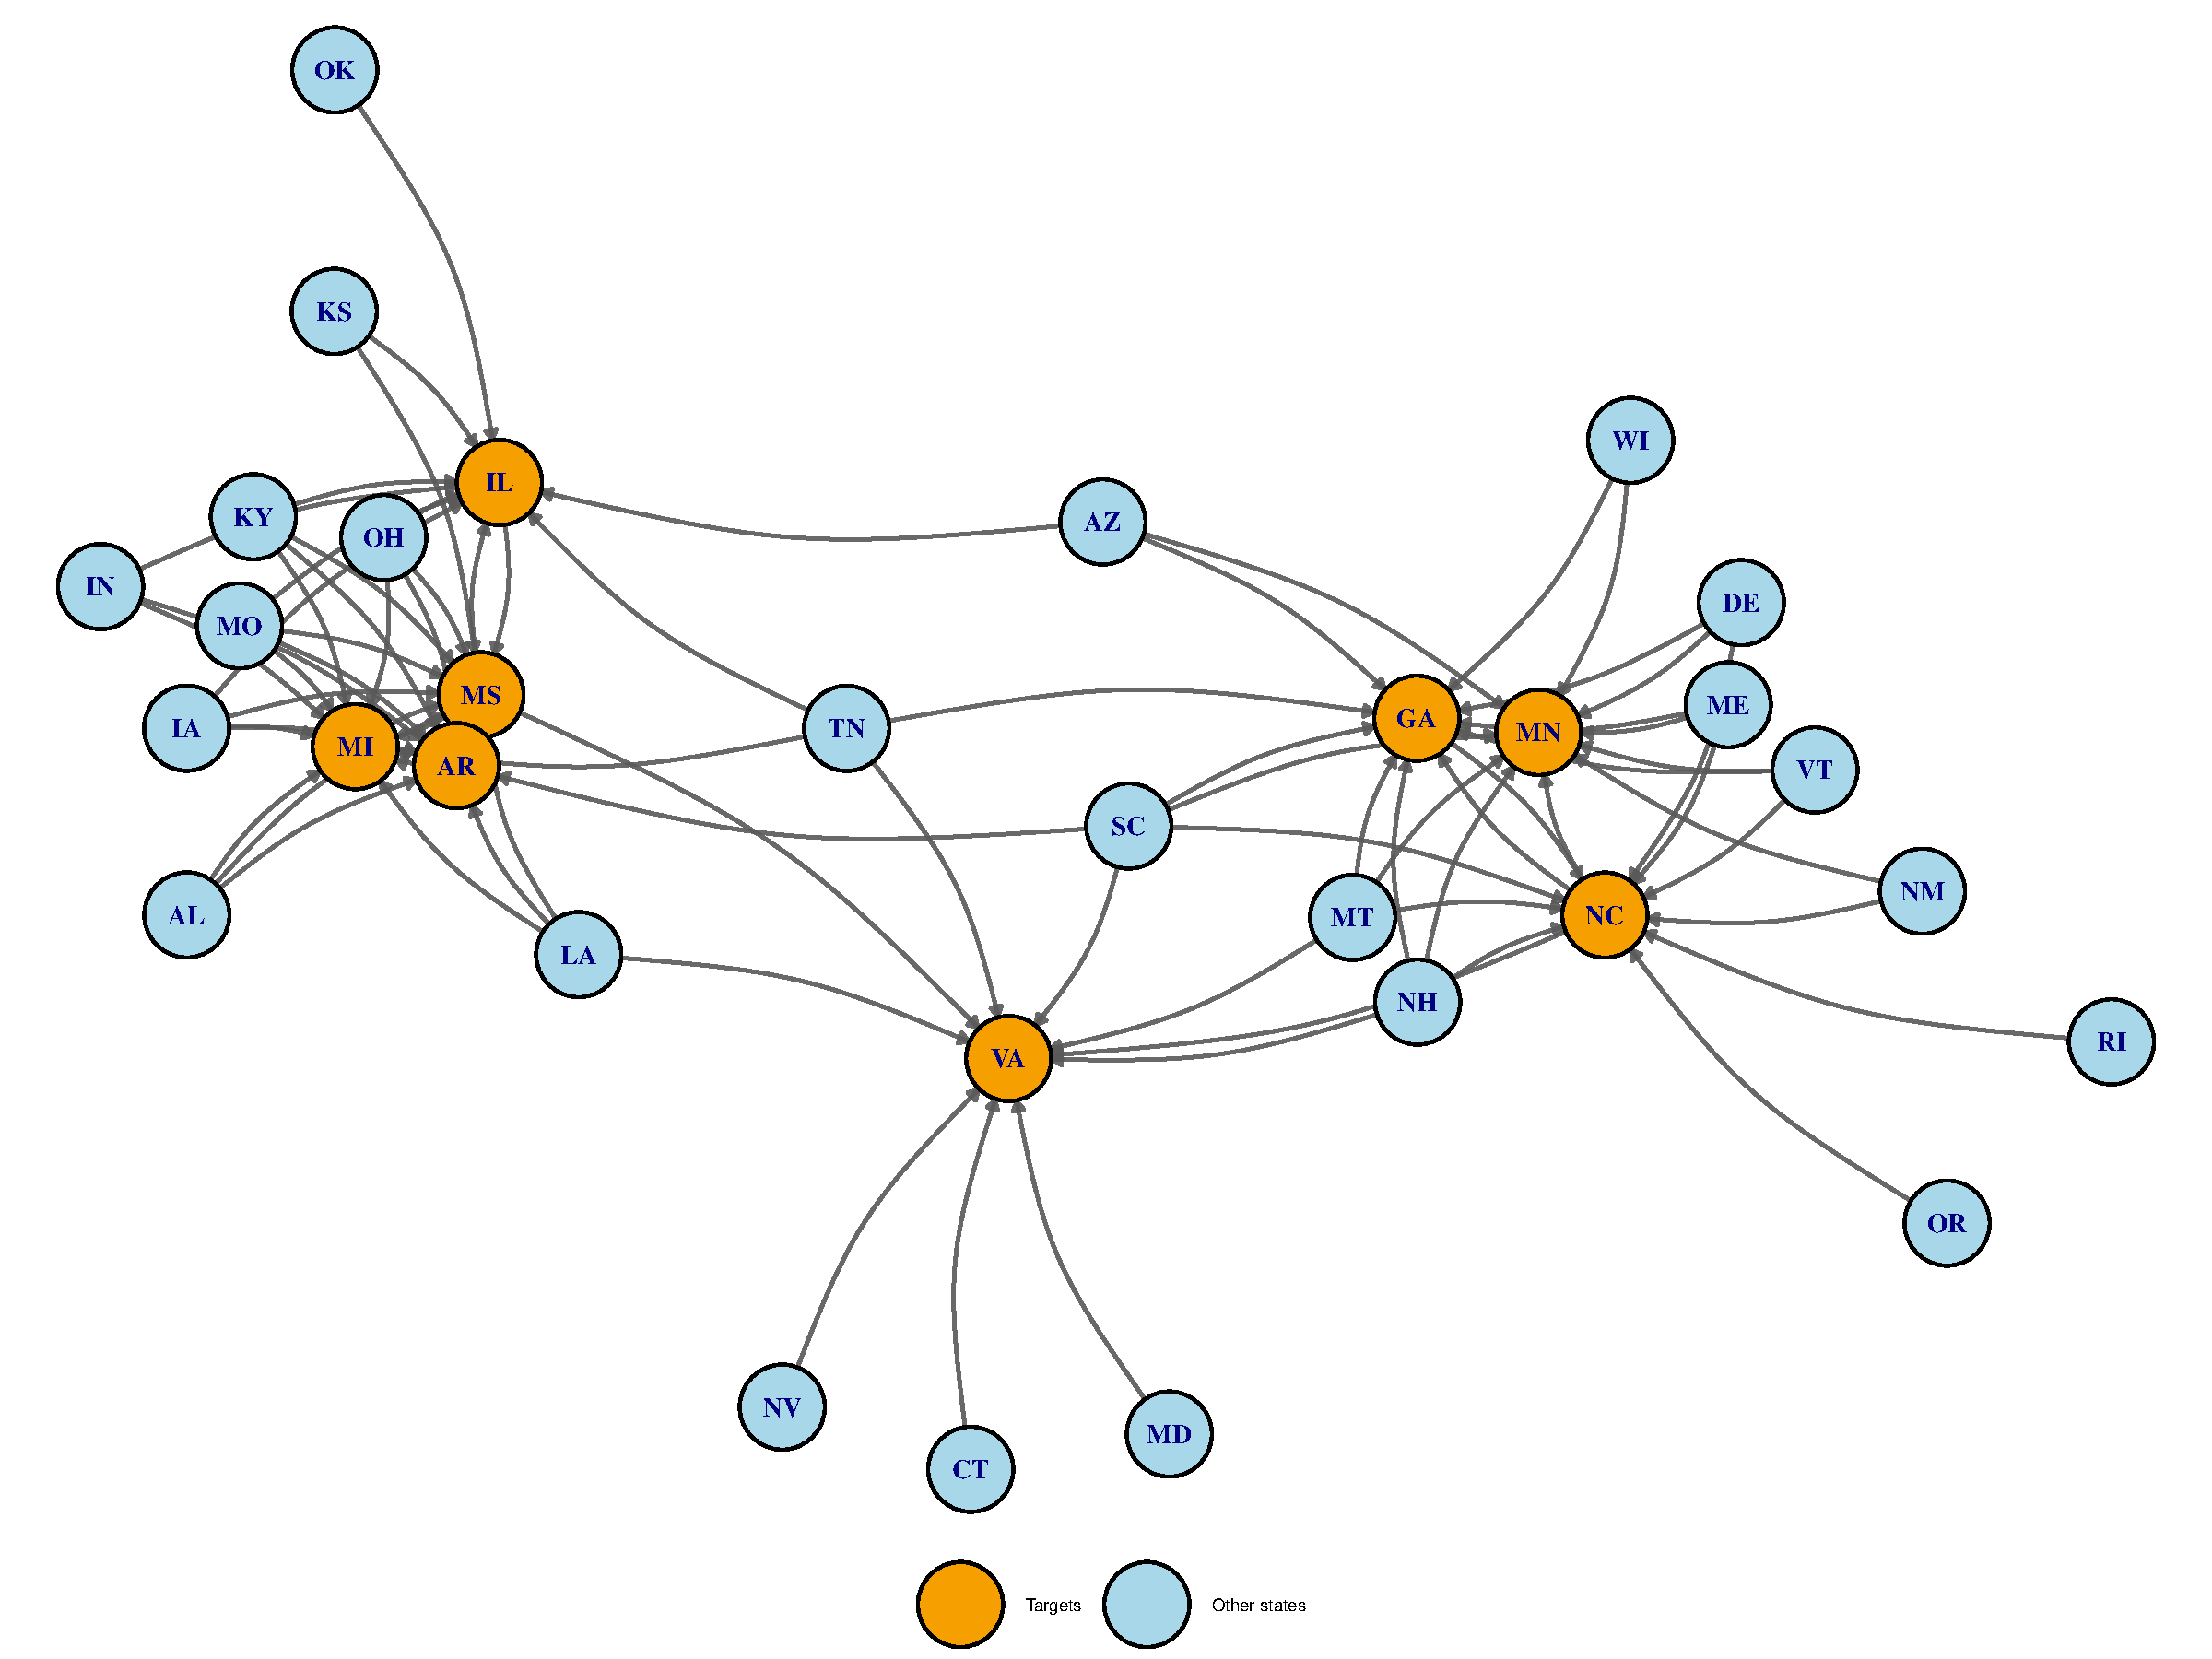
\includegraphics[width=\linewidth]{plots/rda_transfer_top10_con.pdf}
    \caption{Continuous outcome: median housing value.}
    \label{fig:rda_transfer_con}
\end{subfigure}

\vspace{0.8em}

\begin{subfigure}[t]{0.6\linewidth}
    \centering
    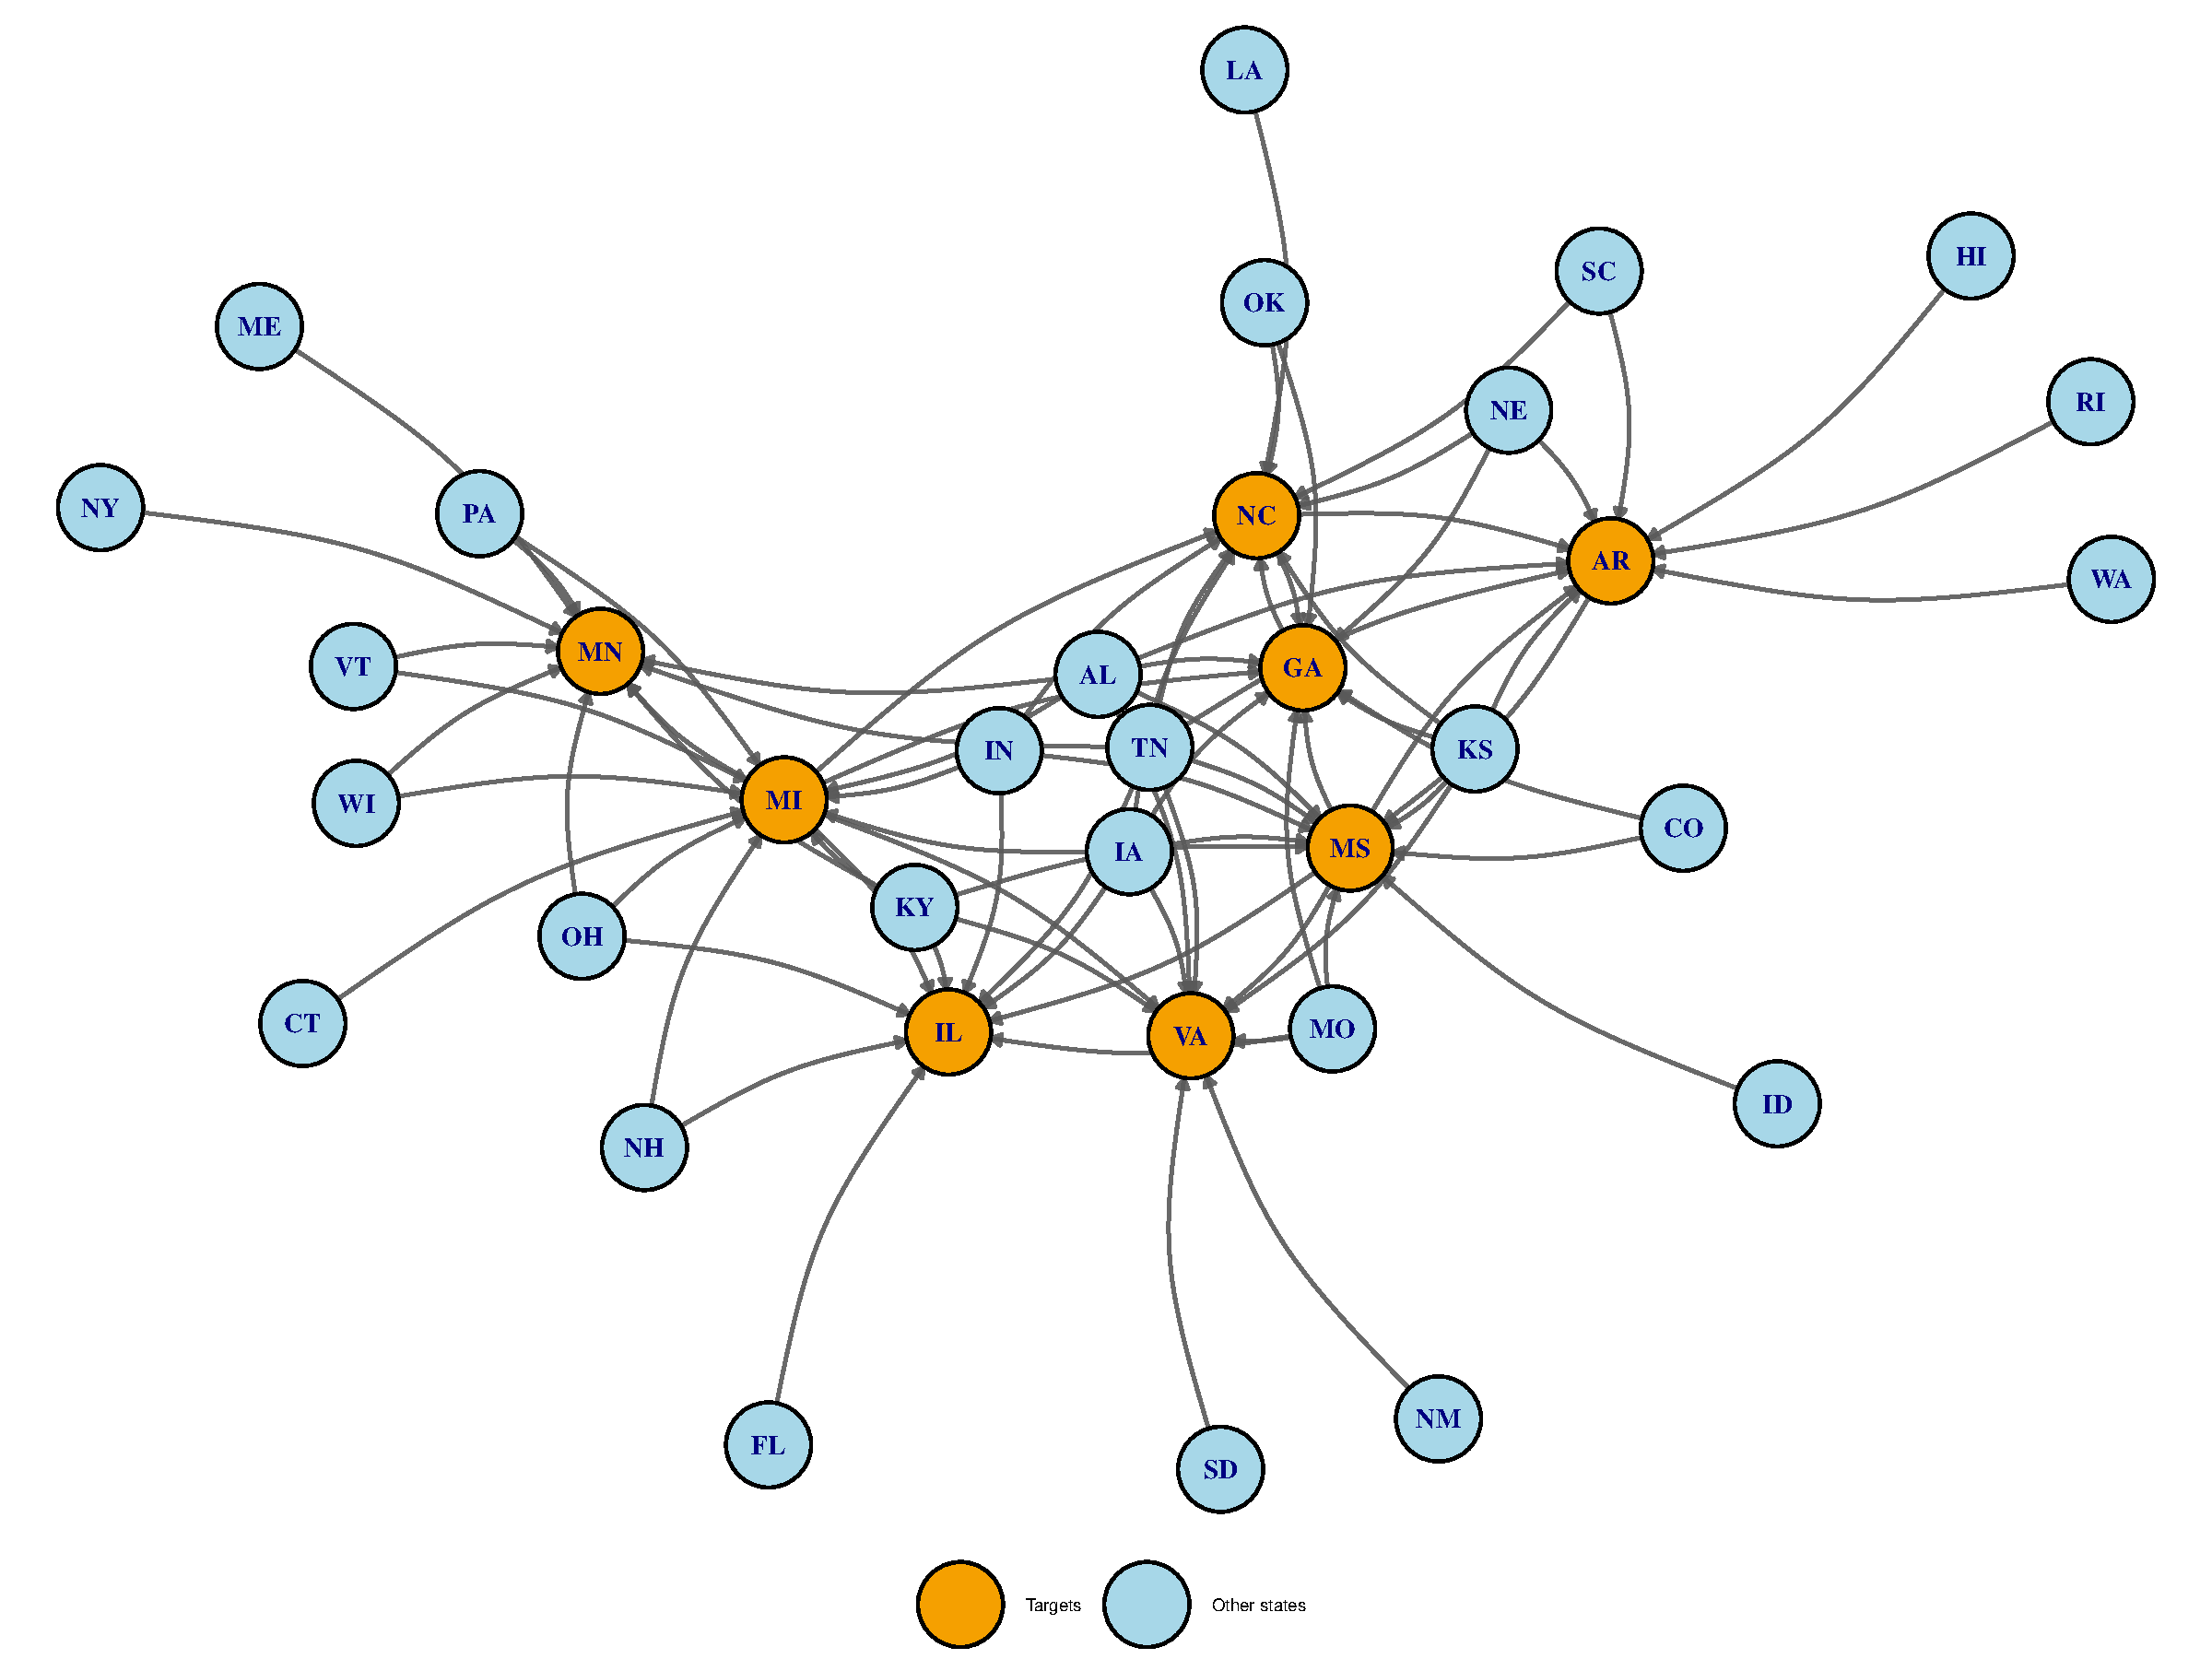
\includegraphics[width=\linewidth]{plots/rda_transfer_top10_cat.pdf}
    \caption{Binary outcome: multi-unit housing $\ge 10\%$.}
    \label{fig:rda_transfer_bin}
\end{subfigure}

\caption{Transferability networks from Trans-GLM. We treat each state as a task and run Trans-GLM source detection for each target state $k$. Orange nodes denote the target states (AR, GA, IL, MI, MN, MS, NC, VA), and blue nodes denote candidate source states. Panel (a) shows the network for the continuous evaluation variable, median housing value, and panel (b) shows the network for the binary evaluation variable, multi-unit housing $\ge 10\%$.}
\label{fig:rda_transfer_both}
\end{figure*}


\section{Discussion and Conclusion}
\label{sec:discussion}

In this article, we propose MTL-MICE and MTL-MICE+, extensions of MICE for multi-task learning in situations where the data sets are similar in variables but differ in their conditional relationships. Transfer learning is applied in each MICE model’s condition to fit the imputation model. Trans-GLM finds a set to transfer by minimizing target held-out loss, and $\mathcal{A}$-Trans-GLM is then used to estimate the pooled coefficients, with an optional target-specific adjustment. MTL-MICE uses the pooled coefficients to impute, while MTL-MICE+ uses the corrected coefficients. To estimate predictive noise for continuous variables, we use an out-of-bag variance estimator according to the 0.632 bootstrap rule, which can prevent under-dispersed imputations that can occur with training-based variance estimation after shrinkage.

In both simulations and the election application, transfer improves imputation accuracy and coefficient recovery, with decreasing benefits as the tasks become less similar. Naive pooling performs poorly in the presence of heterogeneity, especially in the presence of clustered structure or outliers. Trans-GLM source detection, by removing harmful sources, is able to reduce negative transfer effects. The correction step is most beneficial when the selected sources are close to, but not perfectly aligned with, the target. In cases where source detection already finds a very homogeneous set, however, the same step can also increase variance.

Transferability also depends on the type of variables. Continuous variables increase more under high transferability but deteriorate more quickly under mismatch, while binary variables increase more slowly but allow a wider range of transferable sources. In real-world data transfer networks, the continuous housing value exhibits a more regional link pattern, while the binary multi-unit exhibits a more dispersed pattern, as might be expected based on the conditional relationships.

The MTL-MICE framework improves imputation in high-dimensional multi-task settings, but several limitations remain. The current version is built around penalized regression models, and our analysis is limited to continuous and binary variables. However, incorporating multi-categorical variables with multinomial models or dummy coding can significantly increase the problem's dimensionality and make tuning the model difficult. It is computationally expensive when the number of tasks $K$ and variables $p$ is high, as it requires performing source detection and fitting the transfer model within the MICE procedure. However, in practice, it can be reduced using various methods like caching sets, updating them less often, and using coarse filters like sample size and region before performing the detection procedure. The current implementation of MTL-MICE assumes a shared variable set across tasks. However, in cases where feature sets differ across tasks, additional methods are needed to align or share variables among tasks, for example, using transfer models for overlapping covariates and missing variables separately.

However, for inference in the data after multiple imputation, compatibility between the imputation and analysis model is also required. A deeper theoretical treatment of the validity of Rubin rules for selective transfer and repeated correction is beyond the scope of this paper. Future work could prioritize developing adaptive rules for choosing between source detection and correction, incorporating privacy constraints, and evaluating estimands beyond imputation error.

MTL-MICE and MTL-MICE+ extend selective transfer to chained equation multiple imputation by adding transferable source detection and a target correction step, and utilize bootstrap-based uncertainty estimation and out-of-bag variance estimation for continuous outcome data. Simulations and the county election example demonstrate the effectiveness of the approach in terms of accuracy when tasks are similar and stability in the presence of heterogeneity, with different transferability characteristics for continuous and binary outcome data. Based on the results, the best approach is selective multi-task imputation. By treating the decision of whether to transfer as a task-specific rather than a default dataset-wide decision, the approach is more stable in performance across heterogeneous tasks. MTL-MICE and MTL-MICE+ offer a formal approach to the problem of multiple imputation in the chained equation framework that is based on the approach of selective transfer.

\clearpage
\bibliographystyle{agsm}
%\bibliographystyle{wileyNJD-AMA}
\bibliography{references}

\newpage
\begin{center}
{\Large\bf Supplementary Materials}
\end{center}
\label{sec:supplementary}
\setcounter{page}{1}
\setcounter{section}{0}
\renewcommand{\thesection}{S.\arabic{section}}
\renewcommand{\thesubsection}{S.\arabic{section}.\arabic{subsection}}
\setcounter{figure}{0}
\renewcommand{\thefigure}{S.\arabic{figure}}
\setcounter{table}{0}
\renewcommand{\thetable}{S.\arabic{table}}

\section{Detailed Algorithms}
\subsection{MICE}
\begin{algorithm}[H]
\footnotesize
\caption{Multiple Imputation by Chained Equations (MICE)}
\label{alg:mice}
\textbf{Input:} Incomplete data matrix $\bm{X}\in\mathbb{R}^{n\times p}$, number of imputations $M$, number of iterations $T$.\\
\textbf{Output:} $M$ completed datasets $\{\bm{X}^{(q)}\}_{q=1}^M$.
\begin{algorithmic}[1]
\State Initialize missing values in $\bm{X}$ to obtain $\bm{X}^{(0)}$.
\State For each $j\in\{1,\dots,p\}$, let $\mathcal{O}_j=\{i:R_{ij}=1\}$ and $\mathcal{M}_j=\{i:R_{ij}=0\}$ be the observed and missing indices for variable $j$ (fixed across iterations).
\For{$q=1$ to $M$}
  \State Set $\bm{X}^{(q,0)}\leftarrow \bm{X}^{(0)}$.
  \For{$t=1$ to $T$}
    \For{$j=1$ to $p$}
      \State Let $\bm{X}^{(q,t)}_{-j}$ denote $\bm{X}^{(q,t-1)}$ with column $j$ removed.
      \State Fit a conditional model $f_j$ using $(\bm{X}^{(q,t-1)}_{-j}[\mathcal{O}_j],\ \bm{X}_j[\mathcal{O}_j])$.
      \State Draw model parameters $\theta_j$ from the fitted model (e.g., posterior draw or bootstrap draw).
      \State Draw missing values from the predictive distribution:
      \[
        \bm{X}^{(q,t)}_j[\mathcal{M}_j]\leftarrow \text{draw from } f_j\!\left(\bm{X}^{(q,t-1)}_{-j}[\mathcal{M}_j];\theta_j\right).
      \]
      \State Keep observed entries fixed: $\bm{X}^{(q,t)}_j[\mathcal{O}_j]\leftarrow \bm{X}_j[\mathcal{O}_j]$.
    \EndFor
  \EndFor
  \State Set $\bm{X}^{(q)}\leftarrow \bm{X}^{(q,T)}$.
\EndFor
\State \textbf{Output} $\{\bm{X}^{(q)}\}_{q=1}^M$.
\end{algorithmic}
\end{algorithm}

\subsection{$\mathcal{A}$-Trans-GLM}

\begin{algorithm}[H]
\footnotesize
\caption{$\mathcal{A}$-Trans-GLM}
\label{alg:atransglm}
\textbf{Input:} Target data $(\bm{X}^{(0)},\bm{y}^{(0)})$; source data $\{(\bm{X}^{(k)},\bm{y}^{(k)})\}_{k\in\mathcal{A}}$;
penalties $\lambda_w$ and $\lambda_\delta$; cumulant function $\psi(\cdot)$.\\
\textbf{Output:} Estimated target coefficient vector $\hat{\bm{\beta}}$.
\begin{algorithmic}[1]
\State Let $n_0$ be the target sample size and $n_{\mathcal{A}}=\sum_{k\in\mathcal{A}} n_k$.
\State \textbf{Transferring step:}
\[
\hat{\bm{w}}^{\mathcal{A}} \leftarrow \arg\min_{\bm{w}}
\left\{
\frac{1}{n_0+n_{\mathcal{A}}}\sum_{k\in\{0\}\cup\mathcal{A}}
\left[-(\bm{y}^{(k)})^\top \bm{X}^{(k)} \bm{w}+\sum_{i=1}^{n_k}\psi\!\left((\bm{x}^{(k)}_i)^\top \bm{w}\right)\right]
+\lambda_w\|\bm{w}\|_1
\right\}.
\]
\State \textbf{Target correction step:}
\[
\hat{\bm{\delta}}^{\mathcal{A}} \leftarrow \arg\min_{\bm{\delta}}
\left\{
-\frac{1}{n_0}(\bm{y}^{(0)})^\top \bm{X}^{(0)}(\hat{\bm{w}}^{\mathcal{A}}+\bm{\delta})
+\frac{1}{n_0}\sum_{i=1}^{n_0}\psi\!\left((\bm{x}^{(0)}_i)^\top (\hat{\bm{w}}^{\mathcal{A}}+\bm{\delta})\right)
+\lambda_\delta\|\bm{\delta}\|_1
\right\}.
\]
\State Set $\hat{\bm{\beta}}\leftarrow \hat{\bm{w}}^{\mathcal{A}}+\hat{\bm{\delta}}^{\mathcal{A}}$.
\State \textbf{Output} $\hat{\bm{\beta}}$.
\end{algorithmic}
\end{algorithm}

\newpage

\subsection{Trans-GLM source detection for a single conditional model}
% =========================
%  (A) Trans-GLM detection
% =========================
\begin{algorithm}[H]
\footnotesize
\caption{Trans-GLM source detection for a single conditional model $(k,j)$}
\label{alg:transglm_detect}
\textbf{Input:} Target complete-case data $(\bm{Z}^{(k)}_j,\bm{y}^{(k)}_j)$ on index set $\mathcal{O}^{(k)}_j$;
candidate sources $\{(\bm{Z}^{(\ell)}_j,\bm{y}^{(\ell)}_j)\}_{\ell\neq k}$;
GLM cumulant $\psi(\cdot)$; detection penalties $\{\lambda_{\mathrm{det}}^{(0)[r]},\lambda_{\mathrm{det}}^{(\ell)[r]}\}$;
threshold constants $(C_0,\epsilon_0)$.\\
\textbf{Output:} detected transferable set $\widehat{\mathcal{A}}^{(k)}_j\subseteq\{1,\dots,K\}\setminus\{k\}$.
\begin{algorithmic}[1]
\State Randomly split $\mathcal{O}^{(k)}_j$ into 3 folds $\mathcal{F}_1,\mathcal{F}_2,\mathcal{F}_3$.
\For{$r\in\{1,2,3\}$}
  \State $\mathcal{T}_r \leftarrow \mathcal{O}^{(k)}_j\setminus \mathcal{F}_r$.
  \State \textbf{Target-only fit} on $\mathcal{T}_r$:
  \[
    \hat{\bm{\beta}}^{(0)[r]} \leftarrow
    \arg\min_{\bm{\beta}}
    \Bigg\{
      \frac{1}{|\mathcal{T}_r|}
      \sum_{i\in\mathcal{T}_r}\Big[-y^{(k)}_{j,i}\,\bm{z}^{(k)\top}_{j,i}\bm{\beta}+\psi\!\big(\bm{z}^{(k)\top}_{j,i}\bm{\beta}\big)\Big]
      +\lambda_{\mathrm{det}}^{(0)[r]}\|\bm{\beta}\|_1
    \Bigg\}.
  \]
  \For{each source $\ell\neq k$}
    \State \textbf{Single-source pooled transferring-step fit} (no correction):
    \[
      \hat{\bm{\beta}}^{(\ell)[r]} \leftarrow
      \arg\min_{\bm{\beta}}
      \Bigg\{
        \frac{1}{|\mathcal{T}_r|+|\mathcal{O}^{(\ell)}_j|}
        \sum_{i\in\mathcal{T}_r}\Big[-y^{(k)}_{j,i}\,\bm{z}^{(k)\top}_{j,i}\bm{\beta}+\psi\!\big(\bm{z}^{(k)\top}_{j,i}\bm{\beta}\big)\Big] \]
        \[+\frac{1}{|\mathcal{T}_r|+|\mathcal{O}^{(\ell)}_j|}
        \sum_{i\in\mathcal{O}^{(\ell)}_j}\Big[-y^{(\ell)}_{j,i}\,\bm{z}^{(\ell)\top}_{j,i}\bm{\beta}+\psi\!\big(\bm{z}^{(\ell)\top}_{j,i}\bm{\beta}\big)\Big]
        +\lambda_{\mathrm{det}}^{(\ell)[r]}\|\bm{\beta}\|_1
      \Bigg\}.
    \]
    \State \textbf{Validation losses} on fold $\mathcal{F}_r$:
    \[
      \widehat{L}_0^{[r]}(\hat{\bm{\beta}}^{(\ell)[r]})
      =\frac{1}{|\mathcal{F}_r|}\sum_{i\in\mathcal{F}_r}
      \Big[-y^{(k)}_{j,i}\,\bm{z}^{(k)\top}_{j,i}\hat{\bm{\beta}}^{(\ell)[r]}+\psi\!\big(\bm{z}^{(k)\top}_{j,i}\hat{\bm{\beta}}^{(\ell)[r]}\big)\Big],
    \]
    \[
      \widehat{L}_0^{[r]}(\hat{\bm{\beta}}^{(0)[r]})
      =\frac{1}{|\mathcal{F}_r|}\sum_{i\in\mathcal{F}_r}
      \Big[-y^{(k)}_{j,i}\,\bm{z}^{(k)\top}_{j,i}\hat{\bm{\beta}}^{(0)[r]}+\psi\!\big(\bm{z}^{(k)\top}_{j,i}\hat{\bm{\beta}}^{(0)[r]}\big)\Big].
    \]
  \EndFor
\EndFor
\State Aggregate losses:
\[
\widehat{L}_0^{(\ell)}=\frac{1}{3}\sum_{r=1}^3 \widehat{L}_0^{[r]}(\hat{\bm{\beta}}^{(\ell)[r]}),\qquad
\widehat{L}_0^{(0)}=\frac{1}{3}\sum_{r=1}^3 \widehat{L}_0^{[r]}(\hat{\bm{\beta}}^{(0)[r]}).
\]
\State Estimate target-only fold variability:
\[
\hat{\sigma}=\sqrt{\frac{1}{2}\sum_{r=1}^3\Big(\widehat{L}_0^{[r]}(\hat{\bm{\beta}}^{(0)[r]})-\widehat{L}_0^{(0)}\Big)^2 }.
\]
\State Select sources:
\[
\widehat{\mathcal{A}}^{(k)}_j \leftarrow
\Big\{\ell\neq k:\ \widehat{L}_0^{(\ell)}-\widehat{L}_0^{(0)}\le C_0(\hat{\sigma}\vee \epsilon_0)\Big\}.
\]
\end{algorithmic}
\end{algorithm}


\subsection{Outer loop of MTL-MICE/MTL-MICE+}

% ==========================================
%  (D) Outer loop (short)
% ==========================================
\begin{algorithm}[H]
\footnotesize
\caption{MTL-MICE / MTL-MICE+ outer loop (calls Alg.~\ref{alg:one_update})}
\label{alg:mtlmice_outer}
\textbf{Input/Output:} same as Algorithm~\ref{alg:one_update}, plus tasks $\{\bm{X}^{(k)}\}_{k=1}^K$, imputations $M$, iterations $T$.\\
\textbf{Convention:} $q\in\{1,\dots,M\}$ indexes imputation replicates to avoid confusion with $m=p-s$ incomplete variables.
\begin{algorithmic}[1]
\State For each task $k$ and variable $j$, compute $\mathcal{O}^{(k)}_j,\mathcal{M}^{(k)}_j$.
\State Initialize $\bm{X}^{(k,q,0)}$ by sampling observed values within each column (for all $k$, each $q$).
\For{$q=1$ to $M$}
  \For{$t=1$ to $T$}
    \For{$k=1$ to $K$}
      \For{each $j$ with $\mathcal{M}^{(k)}_j\neq\emptyset$}
        \State Update $\bm{X}^{(k,q,t)}_j[\mathcal{M}^{(k)}_j]$ using Alg.~\ref{alg:one_update}.
      \EndFor
    \EndFor
  \EndFor
  \State Save $\bm{X}^{(k,q)}\leftarrow \bm{X}^{(k,q,T)}$ for all $k$.
\EndFor
\end{algorithmic}
\end{algorithm}

\section{Addtional Results}


\begin{figure}[H]
\centering
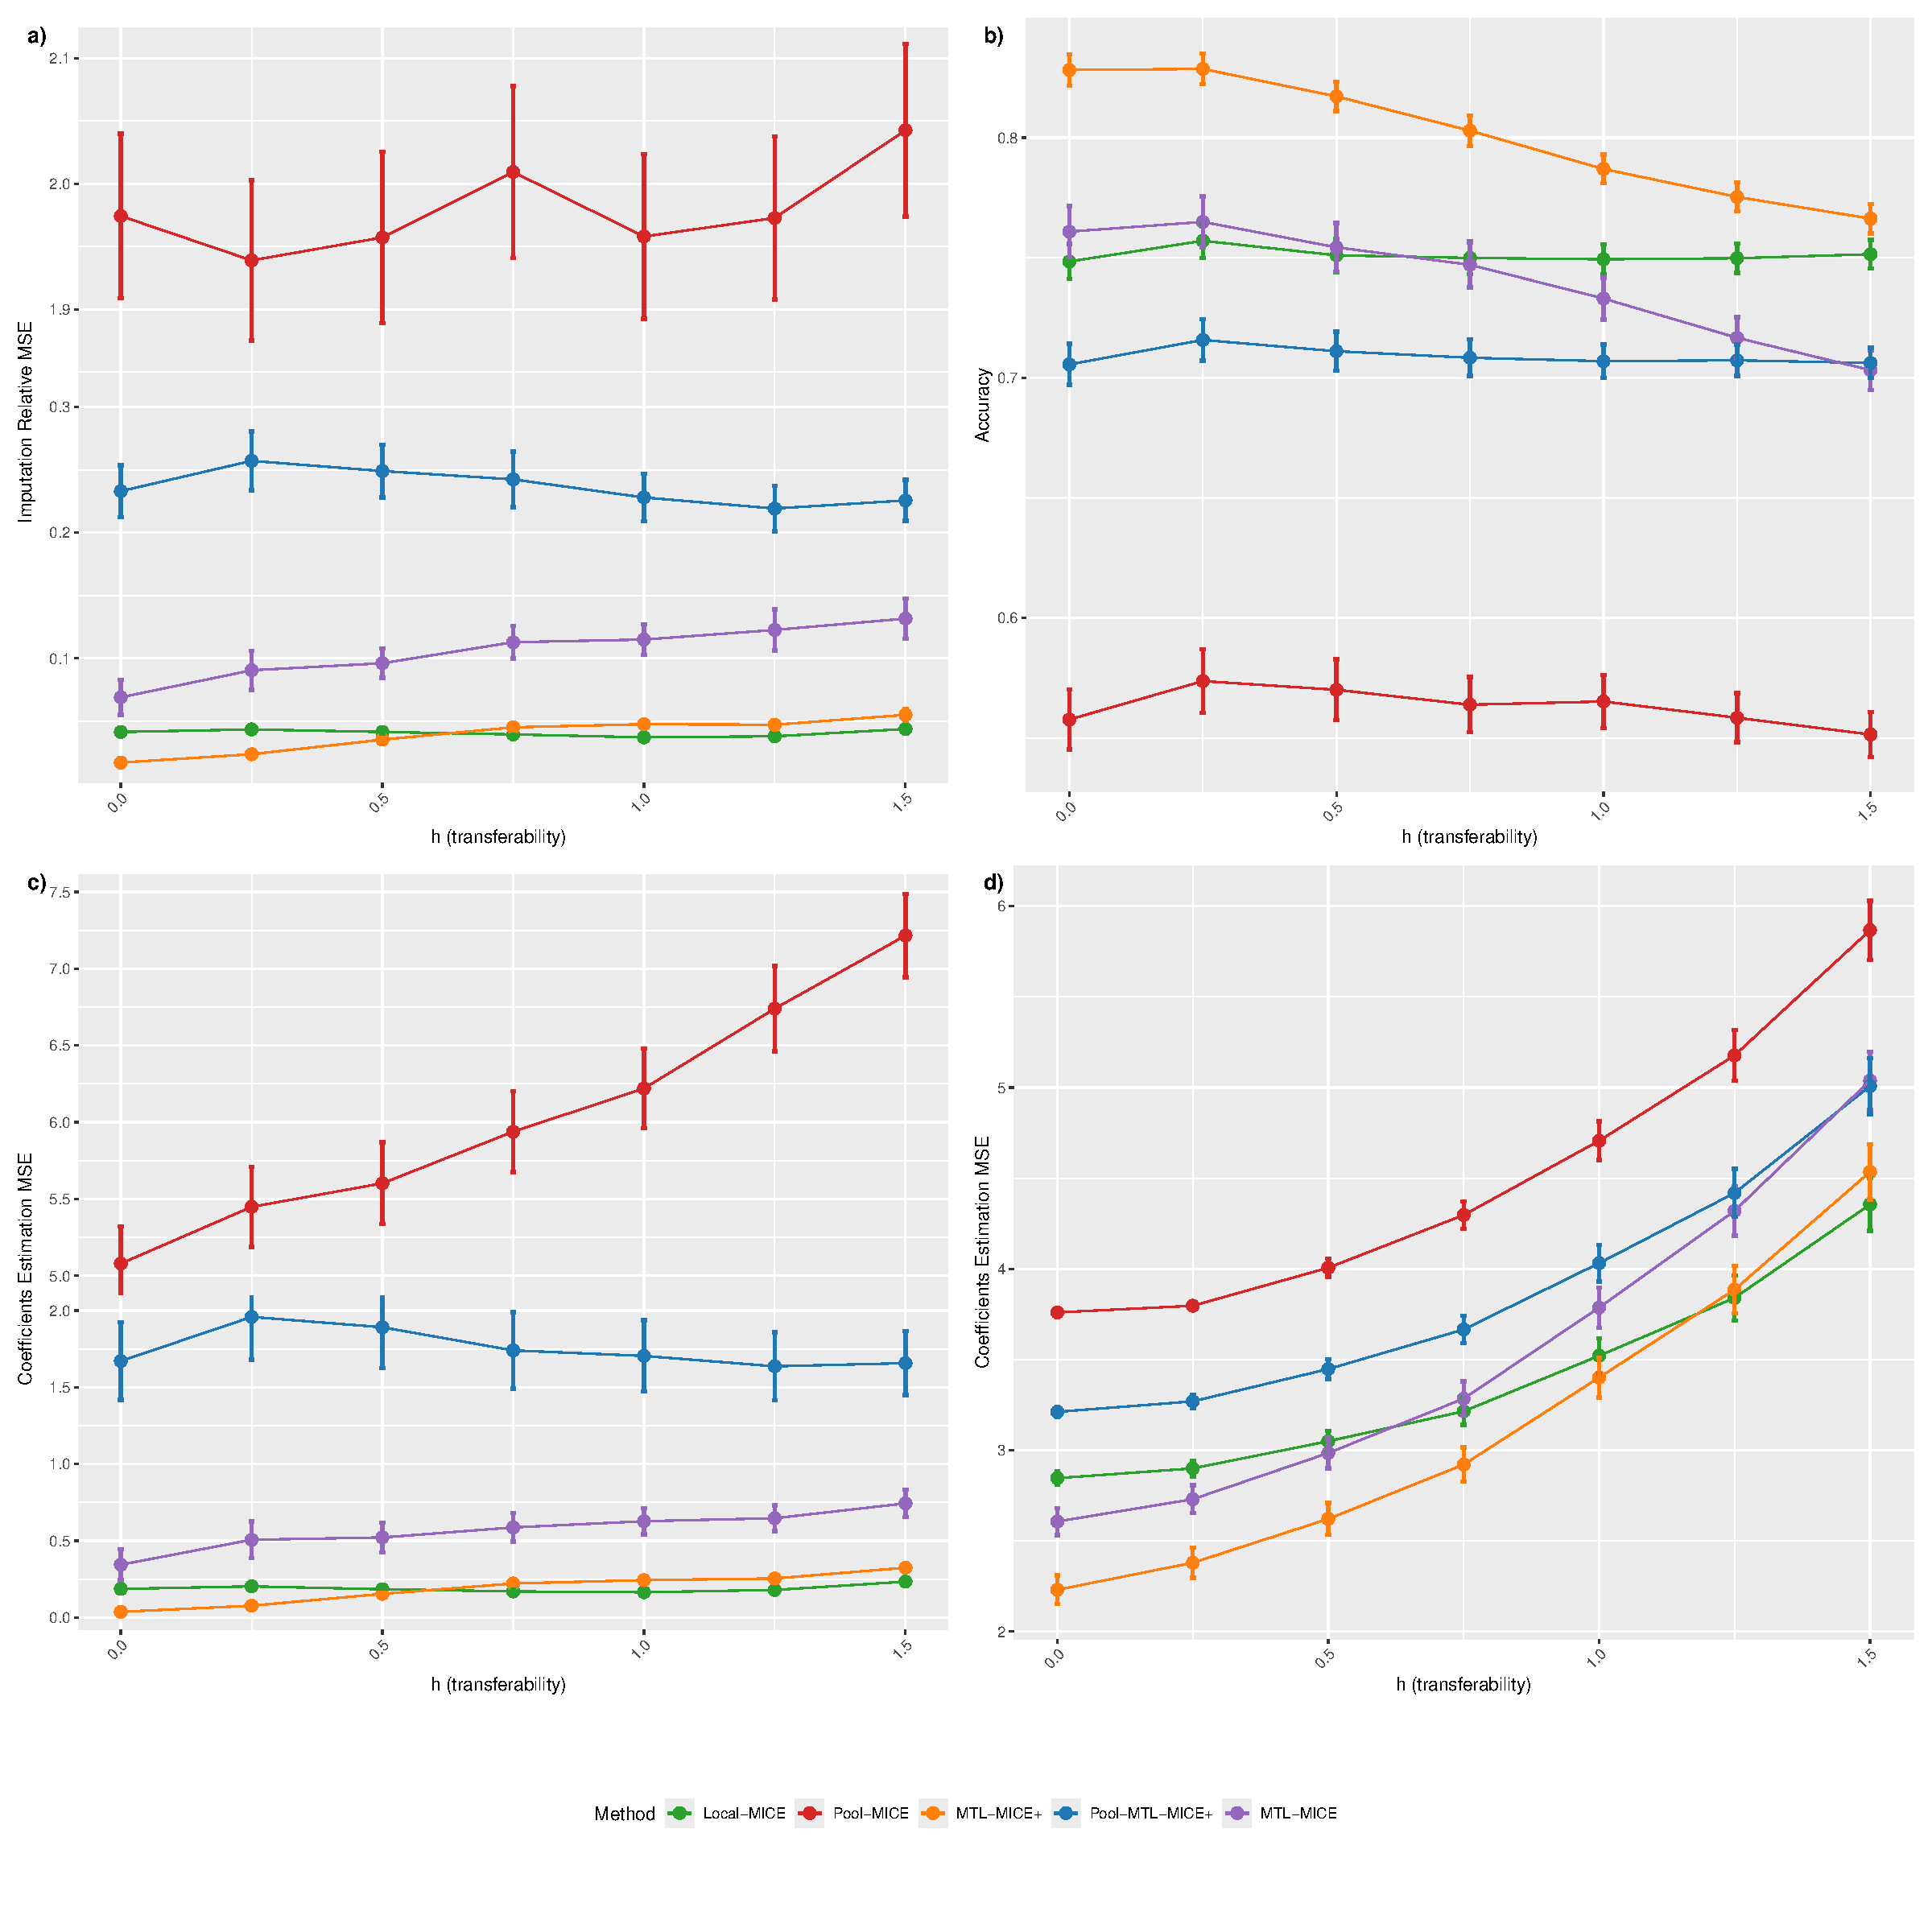
\includegraphics[width=1\linewidth]{plots/sim_htrends_cluster_combined_2x2_1se_2.pdf}

\caption{$h$-trend simulation with clustered tasks (Cluster 2 shown).
Tasks form two symmetric clusters of equal size with opposite coefficient baselines; therefore, Cluster 1 and Cluster 2 produce nearly identical performance curves, and we report Cluster 1 only.
Panels (a)–(b) summarize imputation performance as transferability decreases (larger $h$ implies weaker similarity within cluster), while panels (c)–(d) report coefficient recovery for the corresponding conditional models. Error bars show simulation uncertainty.}
\label{fig:htrend_cluster_2x2_cluster2}
\end{figure}

\begin{figure}[t]
\centering
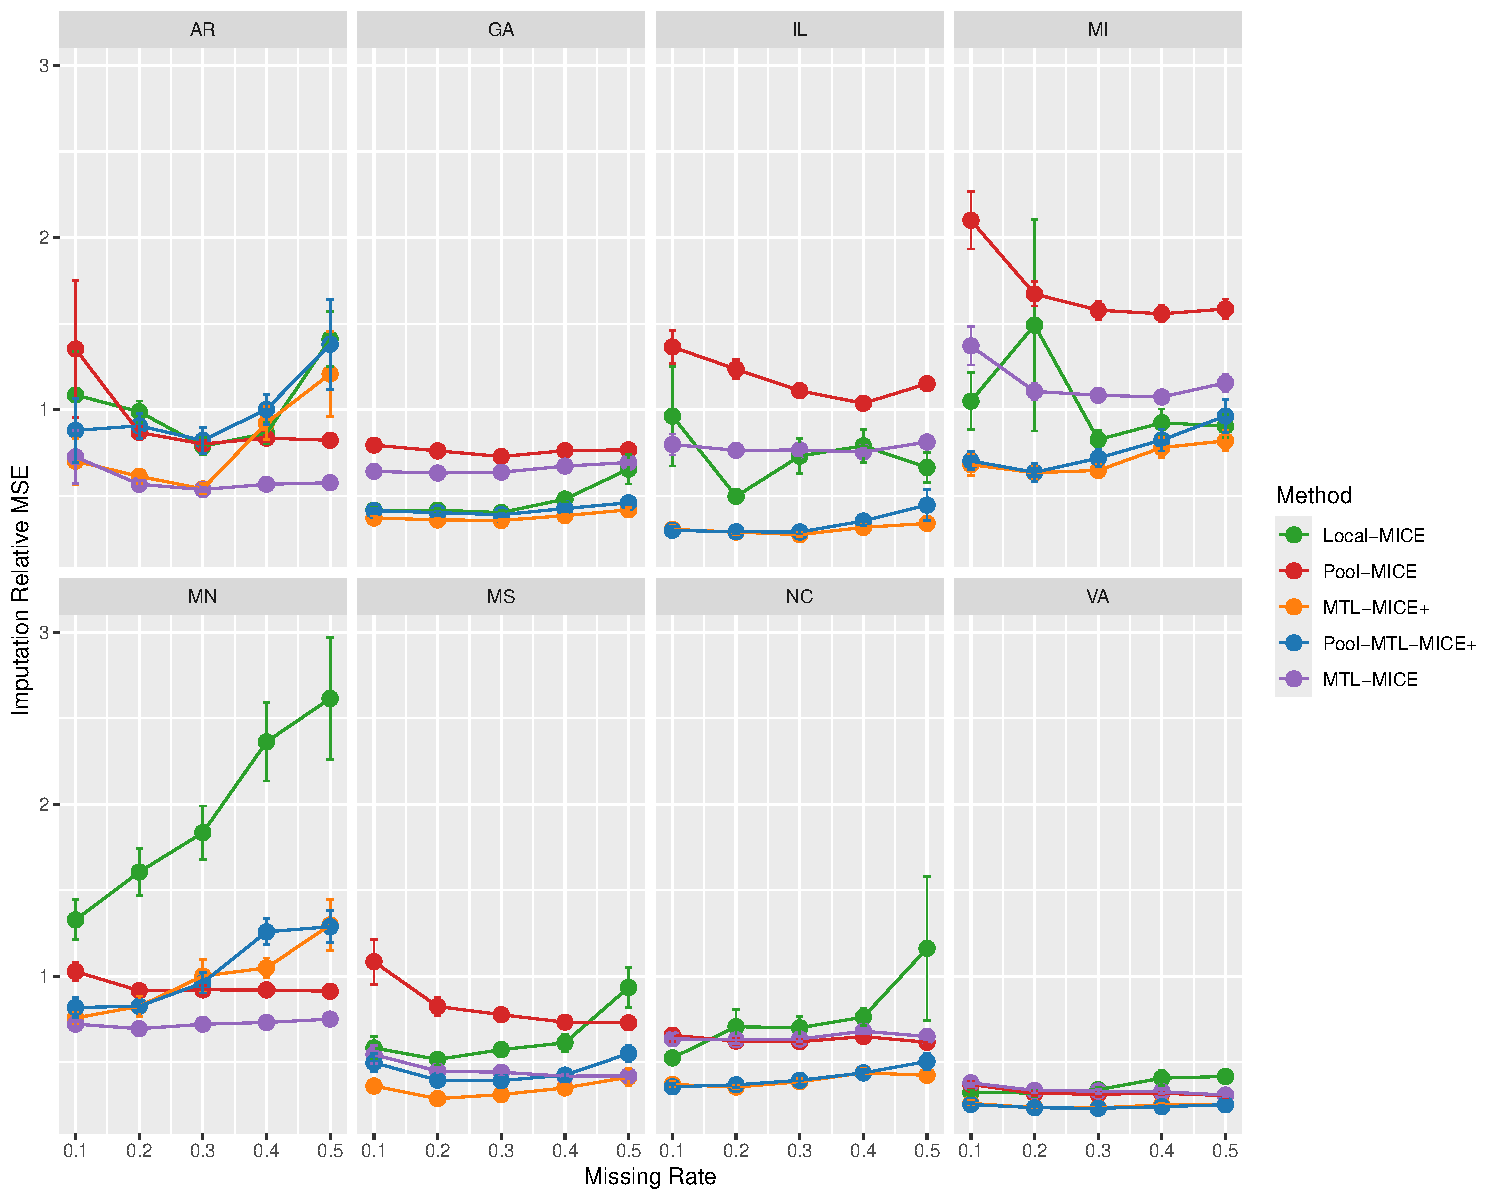
\includegraphics[width=1\linewidth]{plots/rda_uselection_continuous_rss_bystate_plot.pdf}
\caption{Real-data analysis (continuous, by state): county-level 2020 U.S.\ presidential election data.
States are treated as tasks and MAR missingness is introduced at rates
$\rho\in\{10\%,20\%,30\%,40\%,50\%\}$ (averaged over repeated masks).
The plot reports continuous imputation relative MSE, shown separately for each target state;
smaller values indicate better performance.}
\label{fig:rda_cont_bystate}
\end{figure}

\begin{figure}[t]
\centering
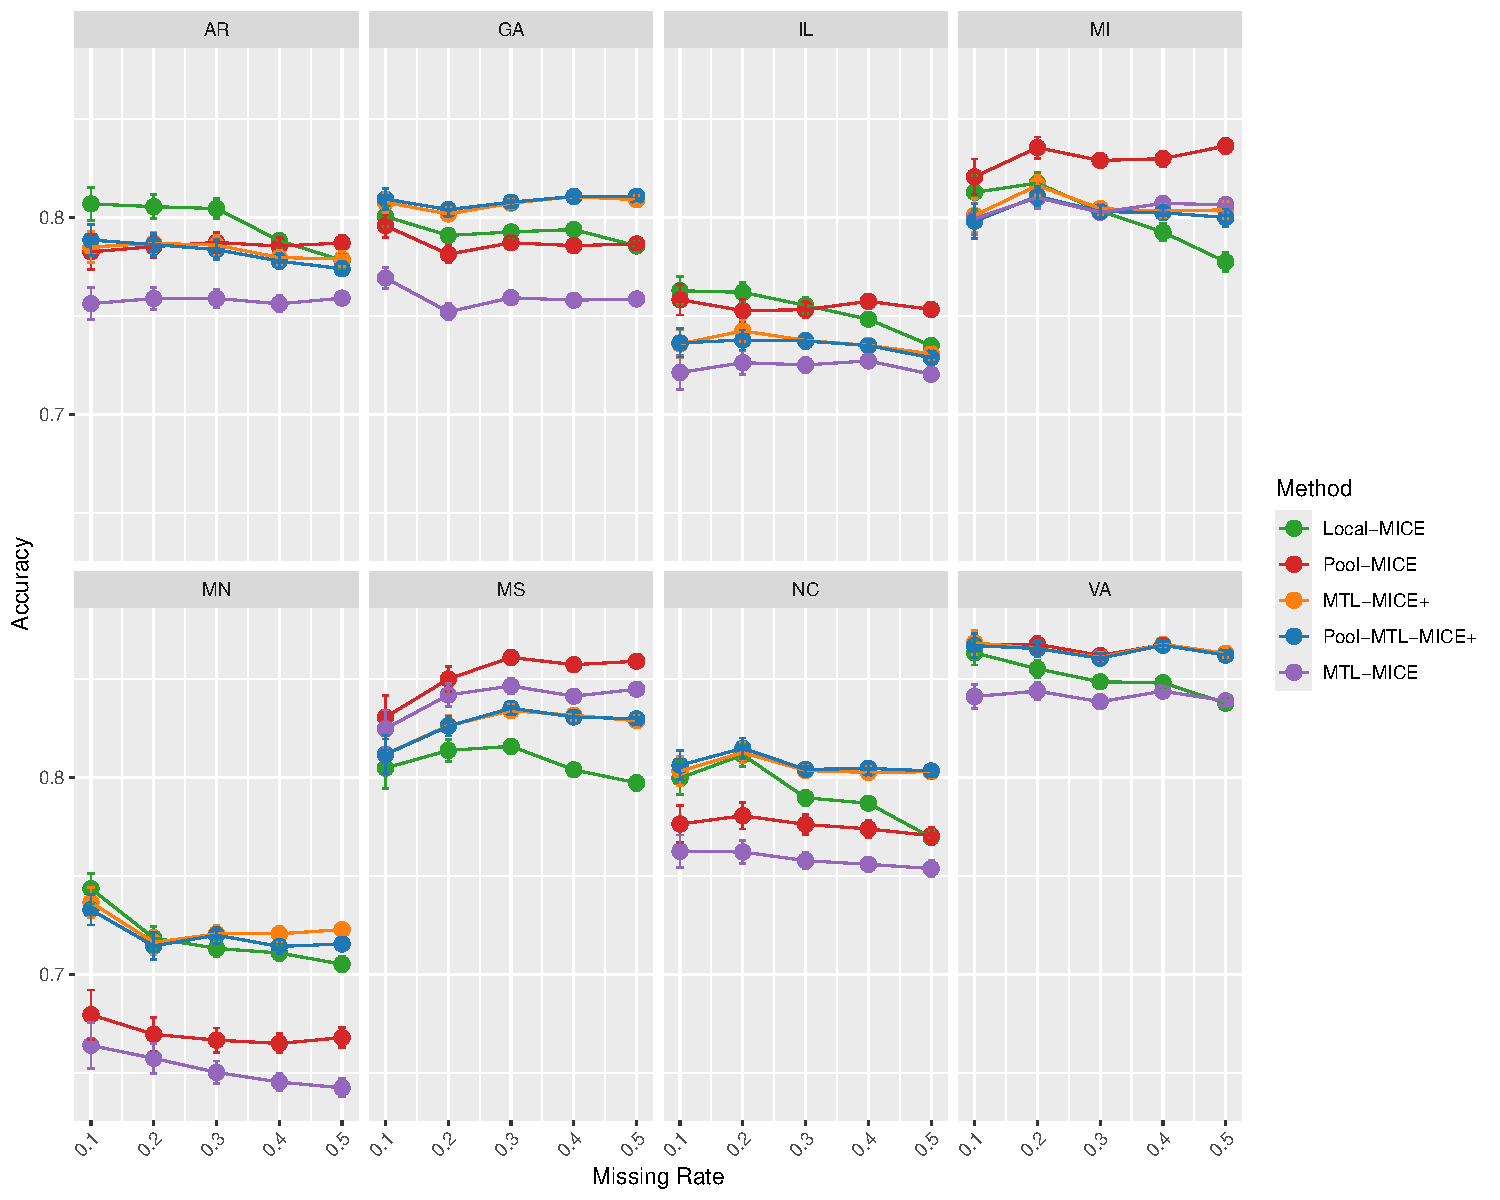
\includegraphics[width=1\linewidth]{plots/rda_uselection_categorical_bystate_plot.pdf}
\caption{Real-data analysis (binary, by state): county-level 2020 U.S.\ presidential election data.
States are treated as tasks and MAR missingness is introduced at rates
$\rho\in\{10\%,20\%,30\%,40\%,50\%\}$ (averaged over repeated masks).
The plot reports accuracy on masked cells for the binary variable (multi-unit housing $\ge 10\%$), shown separately for each target state;
larger values indicate better performance.}
\label{fig:rda_bin_bystate}
\end{figure}



\end{document}